%%%%%%%%%%%%%%%%%%%%%%%%%%%%%%%%%%%%%%%%%%%%%%%%%
%%%%%%%  DUNE COMPUTING MODEL. Start of work October2015.    %%%%%%%%%%%%%%%%
%%%%%%%%%%%%%%%%%%%%%%%%%%%%%%%%%%%%%%%%%%%%%%%%%

\documentclass[12pt]{article}

\topmargin=-0.5in
\oddsidemargin=0in
\evensidemargin=0in
\textwidth=6.2in
\textheight=9.25in

\usepackage[dvips]{graphics}
\usepackage[nomargin,inline,marginclue,draft]{fixme}
\usepackage{rotating}
\usepackage{amssymb,amsmath}
\usepackage{graphicx}
\usepackage{cite}
\usepackage{color}
\usepackage[table]{xcolor}
\usepackage{colortbl}
\usepackage{enumerate}

%\usepackage[titletoc]{appendix}

\usepackage{multirow}

%% draftwatermark causes infinite loop on SL6's ancient TeXLive
\usepackage[firstpage]{draftwatermark}
\usepackage{lipsum}
\usepackage{tikz}

\usepackage[T1]{fontenc}
\usepackage[utf8]{inputenc}
%\usepackage[blocks,affil-it]{authblk}

% experimental - for diameter symbol etc
\usepackage{wasysym}

\RequirePackage{lineno}

\bibliographystyle{plain}
\bibliographystyle{unsrt}

\usepackage{graphicx, subfigure}
\usepackage[colorlinks=true,urlcolor=black,linkcolor=black,citecolor=black,bookmarks=true]{hyperref}

% Depth can be adjusted, and 3 may seem excessive, but when set to 2, a lot of interesting detail in TOC is lost.
\setcounter{tocdepth}{3}


\begin{document}

%\linenumbers

\title{Computing Model for the DUNE Experiment}

\date{\today}

\maketitle

\centerline{The DUNE Collaboration}


\SetWatermarkText{DRAFT}
\SetWatermarkLightness{0.9}
\SetWatermarkScale{3}

\vspace{2cm}

\begin{abstract}
The DUNE Offline Computing Model is described, with  emphasis
on the operations phase of the full DUNE experiment, in which data will
be collected from both a Near Detector located at FNAL and a Liquid Argon TPC
Far Detector located at the SURF laboratory in South Dakota.
Consideration is also given
to earlier computing needs for the design and prototyping phases.  Estimates
are presented for the required storage, CPU, and network bandwidth, and descriptions
of the processing stages and analysis flow are given.  The computing infrastructure
and workflows are designed to meet the approved Computing
Requirements (policies)  of the DUNE Collaboration, which are described.
\end{abstract}



% --- executive summary section ---
\newpage
%\centerline{\textbf{\centerline{\bf{\Large {Executive Summary}}}}} 
%\input{execsum}

%++++++++++++++++++++++++++++++++++++++++
% TOC and lists of tables and figures
\newpage
\tableofcontents
\newpage
\listoftables
\newpage
\listoffigures


%++++++++++++ MAIN DOCUMENT +++++++++++++++
\newpage
\section{Executive Summary}
The Computing Model lays out the general design of DUNE computing infrastructure as well as planning and
organization of its software development effort. It aims to guide the evolution of the DUNE computing
platform in the direction optimal for achieving the scientific goals of the experiment, and will also serve
to inform funding agencies about the scope of work, resource requirements and rate of progress of 
DUNE Software and Computing sector.

After assessment of the characteristics of the data to be generated by the DUNE detector subsystems,
and different data collection modes, it is recognized that DUNE will have to deal with uniquely diverse
types of experimental data which sets it apart from many other experiments (such as collider experiments). More specifically,
the following data streams that will be generated by the DUNE detectors have been identified as having distinct characteristics:
%(with a possible conclustion that they should be collected and processed separately):
\begin{itemize}

\item Data due to interactions of beam neutrinos, cosmic muons and to nucleon decay candidate events in the Far Detector

\item Far Detector data due to candidate Supernova Burst (SNB) events

\item The Near Detector Systems (NDS) data

\end{itemize}

\noindent
The first item corresponds to some of the highest priorities in DUNE, and at the same time it is expected to produce
a very modest amount of data, and at a low rate.

The second item (SNB) necessitates collection of a few candidates
events per year, since the potential rate of real Supernova events, efficiency of the neutrino signal detection
and precise background characteristics are not well known at this point. Thorough understanding of these factors will be crucial
in improvement and fine tuning of the DAQ algorithms necessary for establishing the SNB trigger condition.
Due to necessarily long readout window (in tens of seconds), low thresholds for zero suppression (or even
eschewing zero suppression for better efficiency), and the large number of channels in the TPC this type of events
has a clear potential to dominate the total data volume in DUNE. Since the Supernova Burst candidates are not correlated
in any way with the first item (apart from calibrations that can be done independently), there are no pressing reasons to keep
these data streams together during data transfer and processing.

As far as the Near Detector is concerned, it is massive and expected to produce a sizeable amount of data. It is worth mentioning
that there is no event-level correlation between the Far and Near Detectors. The logistics for moving the data to storage and into processing stage
will also be different for this type of data. Since the Near Detector has a more complex structure than the Far Detector, it has
the potential to require more processing resources for event reconstruction.

In summary, the scale of storage requirements in DUNE will be set according to the strategy chosen for
collection of the Supernova Burst candidate events data. The scale of processing (e.g. CPU requirements)
will be set by the data coming out of the Near Detector Systems. While precise reconstruction of the
\textit{beam neutrino} interactions will be an important challenge in DUNE, in relative terms it will take less storage
and CPU than the other two items.

%It will be optimal to keep the corresponding data streams (which are not directly related to each other) and associated processing
%separate in order to ensure flexible and more agile data placement and efficient use of available CPU power.


\subsection{DUNE}

The Deep Underground Neutrino Experiment (DUNE) will provide a unique, world-leading program
for the exploration of key questions at the forefront of particle physics and astrophysics~\cite{sciopps}.

DUNE will involve a number of subsystems and components. From the computing
perspective, two can be qualified as especially important:

\begin{enumerate}

\item a fine-grained \textbf{Near Neutrino Detector} just downstream of the neutrino source
\item a massive liquid argon time-projection chamber (LArTPC) deployed as a \textbf{Far
Detector} deep underground, 1,300 km downstream from the source of neutrinos located at FNAL

\end{enumerate}

The Near Detector will comprise a ``fine-gran tracker'' (FGT) and a calorimeter, with channel count of the order of O($10^{5}$).

The Far Detector will be installed at the Sanford Underground Research Facility in Lead, South Dakota.
Its sensitive volume will be formed by a total of 40kt of Liquid Argon instrumented with $\sim$1.5 million readout
channels to detect ionization. It will also incorporate a photon detector which will detect scintillation
signal produced by ionizing patciles traveling in Liquid Argon.



\subsection{About the Computing Model}
\label{sec:modelrole}

The DUNE Computing Model plays central role in the design of the computing infrastructure of the experiment, as well as
planning and organization of its software effort. It aims to guide the evolution of the DUNE computing platform in the direction
optimal for achieving its scientific goals. It will also serve
as an instrument to inform the funding agencies about the scope of work and rate of progress of the DUNE  
Computing Organization.

The Computing Model contains the \textit{Software and Computing Requirements} that define a set of rules and principles by which technologies
are selected and specific practices and policies implemented in DUNE computing. The benefit of having the \textit{Requirements} in place is that they reflect a broad consensus
within the Collaboration regarding what it needs from its computing sector and its components, thus fostering cooperation and better
integrations of systems and components in DUNE.

Another factor that defines the structure and content of the Computing Model are the characteristics of the data to be collected,
processed and otherwise generated in the experiment. For example, raw data rates will dictate the scale and required capabilities
of the Data Acquisition System, which in turn will determine the scale and other characteristics of offline systems required by DUNE.
The scope and projected volume of Monte Carlo studies will set the scale of CPU and storage resources needed.



\subsection{The DUNE Timeline and Evolution of the Computing Model}
According to current plans, DUNE will be commissioned in mid-2020s. The decade before the commissioning will be quite busy
for DUNE, which is currently in the stage of broad and active R\&D effort, supported by the development of appropriate 
software tools in each area. Extensive simulations are being performed to support design decisions pertaining to the Liquid 
Argon TPC as well as a number of other detector elements and subsystems (cf. the proposed Near Detector, the Photon Detector, 
the target complex etc). Background characterization, event reconstruction techniques and studies are systematic errors are all under active development.

Importantly, at the time of writing DUNE is actively working on two LArTPC prototypes:
\begin{itemize}
\item 35t Liquid Argon TPC situated at FNAL which will start taking cosmic ray data in 2016
\item The ``Full Scale'' prototype to be placed in a test beam at CERN, scheduled for commissioning in 2017 and actual data taking in early 2018
\end{itemize}

It follows that although commissioning and operation of the eventual full detector is still years away, DUNE is effectviely engaged
in a vigorous experimental program which poses non-trivial requirements from the computing standpoint. The landscape of DUNE
computing will be defined by these and similar tasks for the next few years.

After the crucial prototyping stage is completed, the workup to start of data taking in DUNE will include scaling up the data management and processing systems,
integration testing,  stress testing and  realistic data challenges preceding the commencement of operations. For this reasons it's obvious that the DUNE
Computing Model will undergo considerable evolution. In the present document, this is addressed  by using the following approximation and structure:

\begin{itemize}

\item The time period between the year 2014 and the commissioning of DUNE (its timing being uncertain as of now but assumed to be around 2026) is divided into two parts of roughly equal duration, i.e. 2014-2020 and 2020-2026. This segments will be referred to as \textbf{T1} and \textbf{T2}.


\item Where warranted, major sections of the Computing Model will contain separate subsections reflecting these two time periods.

\end{itemize}
 
It is obvious that rapid evolution of software and computing technologies, combined with dynamic nature of R\&D in DUNE (and other  projects with potential impact on DUNE) and a variety of other factors makes precise formulation of the Computing Model and subsequent plans very difficult over the foreseen extended timeline. It  therefore likely that it will become necessary to evaluate the Computing Model and make adjustments at some point in time. We estimate that the transition between T1 and T2 periods (i.e. roughly 2020) will be an appropriate point in time to revisit the Computing Mode, develop its next
iteration and adjust the plans derived from it.



\newpage
\section{DUNE Data Characteristics}
\label{sec:data-characteristics}
\subsection{Overview}

A number of parameters from DUNE/LBNF requirements, design documents,  and studies are used  as input
for estimations of the data rates in DUNE.
%In cases when derived parameters need to be generated based on these inputs this is accomplished using
%the software package \textit{dune-params}\cite{duneparams}
%developed specifically for this purpose. As the inputs and estimations are refined the results presented in this annex can be regenerated at will.
Buffering, triggering and readout strategy and algorithms of the DAQ
are complex R\&D items and are far from their final design and state of
readiness at the time of writing. Same applies to various analysis software.
For that reason, the data rate estimations involve some broad assumptions
and leave open some choices. This is described in more detail in the following subsections.

DUNE contains a number of major detector subsystems. The Liquid Argon TPC will present most challenges from
the standoint of real-time data processing and triggering, and can potentially dominate the data volume.
It incorporates the Photon Detector (PD) which while important produces less data so it won't be our focus
for the purpose of the data rate and volume estimates. There is also the Near
Detector Systems (see~\ref{sec:nds-params}).

\subsection{DUNE Detectors and Subsystems}

\subsubsection{Fundamental Parameters of the LArTPC}
\label{sec:fundamental-parameters}

The fundamental TPC parameters most relevant as input to the data rate estimations are summarized in
table~\ref{tab:fundamental-parameters}.

\begin{table}[ht!]
	\centering
	\begin{tabular}{| p{2.5in} | p{1in} |}
		\hline
		\textbf{Parameter} & \textbf{Value} \\ \hline
		Full height (single module) & 12.0\,m \\ \hline
		Full width (single module) & 14.5\,m \\ \hline
		Full length (single module) & 58.0\,m \\ \hline
		\# of detector modules & 4 \\ \hline
		\hline
		channels per APA & 2,560 \\ \hline
		APAs per module & 150 \\ \hline
		Active height (APA) & 6.0\,m \\ \hline
		Active width (APA) & 2.3\,m \\ \hline  \hline
		Drift distance in Liquid Argon & 3.6\.m \\
		\hline
		Drift velocity & 1.6\,mm/$\mu$s \\ \hline
		Drift time & 2.25\,ms \\ \hline
		\# drifts/readout factor & 2.4 \\ \hline
		readout time & 5.4\,ms \\ \hline \hline
		bytes/sample & 1.5 \\ \hline
		sample rate & 2.0\,MHz \\ \hline
		samples/readout & 10,800 \\
		\hline \hline
		Total \# of channels & 1,536,000 \\
		\hline
	\end{tabular}
	\caption{Fundamental parameters of DUNE Far Detector LArTPC.}
	\label{tab:fundamental-parameters}
\end{table}

Two of the parameters listed above (``drifts/readout'' and ``readout time'') need an additional comment.
The nominal readout time of 5.4ms is chosen such that additional time windows are covered just before and just
after the nominal $t_0$ (trigger) window. The value of 5.4\,ms is 2.4 times larger than the nominal drift of 2.25\,ms,
and it's listed in the table as the ``drifts/readout'' factor. This factor is not calculated precisely but was chosen based
on the experience with the 35t prototype (Sec.\ref{sec:35t}). The motivation behind this exta readout it to capture
potential activity in the TPC just before and just after the event of interest, so as to characterize this extraneous
ionization which for example can manifest itself as track segments due to cosmic rays background. It is quite
possible that the readout time will be revised as the final detector design is progressing, however the value of 5.4\,ms
was fixed in this document as nominal, in order to provide consistency of various estimates related to the data.

\subsubsection{The Photon Detector}
\label{sec:pd}
The Photon Detector (PD) which is built into the Far Detector LArTPC takes advantage of the fact that Liquid Argon
is an excellent scintillating medium.
The most significant requirements for the PD include determination of $t_0$ of an event relative to the TPC timing ---
resolution better than 1\,$\mu$s (event position resolution along drift direction of a few mm), and sufficient light
collection efficiency to allow triggering on neutrinos coming from a supernova, with the capability of detecting neutrinos with energies as
low as 20\,MeV.

Light produced by Liquid Argon Stintillation is collected from the TPC volume by the wavelength shifter and transported
by the light guide to the Silicon Photo-Multiplier (SiPMs) mounted at its end. A single whole assembly is mounted on each  APA frame.
The SiPMs are read out using shielded twisted-pair cables and the signal is passed to the module called SSP (the SiPM Signal
Processor). Digitized data is processed by a  Field-Programmable Gate Array (FPGA). The use
of the FPGA processing allows for a significant amount of customization of the SSP operation.


\subsubsection{The Near Detector Systems}
\label{sec:nds-params}
For sake of brevity, only basic information will be provided for the Near Detector Systems (NDS) which are under active development
at the time of writing and for which there is no final design yet. The main NDS components are:
\begin{itemize}
\item Near neutrino detector (NND), and its major component, the Fine-Grained Tracker
\item Beamline Measurement System (BLM)
\end{itemize}
\ 
In the reference design at the time of writing, the Fine-Grained Tracker (FGT) near consists of a straw-tube
tracking detector (STT), $\mu$-identifiers (MuID) and electromagnetic calorimeter (ECAL), all placed inside of a 0.4\,T dipole magnet.

\begin{table}[ht!]
\centering
\begin{tabular}{| p{2in} | p{1.5in} |}		\hline		
\textbf{Item} & \textbf{Specification} \\ \hline
Straw Tube Geometry & $\diameter$1\,cm$\times$3.5\,m length \\ \hline
Number of straw tubes & 107,520\\ \hline
Straw tubes per plane & 336 \\ \hline
Planes per module & 4 \\ \hline
Number of modules & 80 \\ \hline
Number of channels & 215,040 \\ \hline
\end{tabular}
\caption{Main parameters of the FGT}
\label{tab:fgt-params}
\end{table}

The FGT is designed to make precision measurements of the neutrino
fluxes, cross sections, signal and background rates at the percent level. A summary of basic parameters of the
NDS are presented in Table~\ref{tab:nds-params}.
\begin{table}[ht!]
\centering
\begin{tabular}{| p{1in} | p{1in} | p{1in} |}		\hline		
\textbf{Detector} & \textbf{Mass} & \textbf{Channels} \\ \hline
SST & 8t & 215,040 \\ \hline
ECAL & 93t & 52,224 \\ \hline
MuID & 100t & 165,888 \\ \hline
\end{tabular}
\caption{Main parameters of the Near Detector Systems}
\label{tab:nds-params}
\end{table}

The Beamline Measurement System (BLM) will be located in the region of the Absorber Complex
at the downstream end of the decay region to measure the muon fluxes from hadron decay.
It is not anticipated to produce large amounts of data when compared to other detectors in DUNE.

\subsection{The Far Detector LArTPC Data}
\label{sec:fd-data-overview}
\subsubsection{Sources of Data in the TPC}

Data being read out from the TPC are the result of a few different classes of interactions and other phenomena,
as outlined in table~\ref{tab:dune-data-sources}. Characteristics of these sources will
be a major factor influencing the rate and volume of data produced in DUNE.
\begin{table}[ht!]
	\centering
	\begin{tabular}{| p{1in} | p{4.5in} |}
		\hline
	\textbf{Type} & \textbf{Description} \\ \hline
		
	in-spill & Any activity in the detector which is coincident with
	the passage of beam neutrinos through the detector \\ \hline
	
	with-beam-$\nu$ & A subset of \textit{in-spill} where activity is
	consistent with a beam-$\nu$ interacting in the detector \\ \hline
	
	cosmic-$\mu$ & Activity due to the passing of cosmic-ray muons
	through the detector \\ \hline
	
	radioactivity & Activity due to the decay of radioactive
	isotopes \\ \hline
	
	atm-$\nu$ & Activity consistent with interactions from
	atmospheric neutrinos \\ \hline
	
	noise & Electronics noise (common-mode not considered) \\ \hline

	\end{tabular}
	\caption{Sources of data in the LArTPC.}
	\label{tab:dune-data-sources}
\end{table}

Not included in this table are two of the more exotic sources of signal, the Supernova Burst and Nucleon decay.
Due to their rare (and generally speaking, potential) occurance and differing characeristics they will be considered separately
in~\ref{sec:snb-data} and \ref{sec:pdk-data}.

\subsubsection{Segments of the Dynamic Range of the TPC signals}

Signals produced by individual wires in the DUNE TPC will have a substantial
dynamic range. For example, $\beta$-decay of naturally occurring isotope $^{39}$Ar has the endpoint of
565\,keV, whereas signals due to interactions of energetic neutrinos can produce signals
equivalent up to a few MeV energy deposition in a given channel depending on the event topology.

Each segment of the dynamic range will reflect certain types of events and this
be characterized by a respective data rate. For a systematic approach to estimates
and to reflect the physics of the detector, it is helpful to consider three such segments when characterizing the LArTPC data.
To set the scale for these segments we can assign ``thresholds''corresponding to each of them.
The threshold values can be applied to signals on ``per-wire'' basis and defined for example
in terms of ADC values (reflecting the collected charge, which can be translated to units like MeV with proper calibration).
These are not meant to be precise values used in data collection and are given here for orientation purposes only.
Using this concept the dynamic range can be considered with three distinct settings:
\begin{description}
	
\item[full-stream] The full-stream \textbf{(FS)} threshold means \textit{there is no threshold at all}, i.e.
FS data is effectively read out in every time bin (as defined by the ADC clock) and from every channel.

\item[zero-suppressed] The zero-suppression \textbf{(ZS)} threshold is an ADC value (in a single time bin,
on a single wire) roughly corresponding to ionization charge due to a 0.5\,MeV energy deposition.
All bins with ADC counts below this threshold are discarded from the data stream.

\item[high-energy] A high-energy \textbf{(HE)} threshold is assumed to be high enough so that
  that all electronics noise signals from radioactive decays are suppressed but low
  enough to not impact activity from beam neutrino interactions or potential nucleon decay activity.
  Further studies are needed to determine this threshold but currently
  it is taken, without rigor, to be $O(1)$\,MeV.

\end{description}

The categories thus introduced will be considered in more details in the following sections, for example
see \ref{sec:zs-data} for a discussion of Zero Suppression and \ref{sec:ar39decays} for a discussion of
$^{39}$Ar decays rejection.


\subsubsection{Full-stream Data}

Full-stream (FS) data corresponds to reading all data in every ADC channel without
application of any threshold. Estimating the corresponding rate is a calculation based on
known parameters as it does not depend on the activity in the detector or the noise
level of the electronics. As its name implies, it is the most voluminous type of data
that can be generated by the TPC. The parameters which apply to this data are given in
table~\ref{tab:full-stream-parameters}.

\begin{table}[ht!]
	\centering
	\begin{tabular}{| p{3in} | p{1.1in} |}
		\hline

	\textbf{Parameter} & \textbf{Value} \\ \hline
	
	Bytes per sample & 1.5 \\ \hline
	
	DAQ sample rate & 2.0\,Mhz \\ \hline
	
	Channels per APA & 2,560 \\ \hline
	
	Number of APA per detector module & 150 \\ \hline
	
	Number of modules & 4 \\ \hline
	
	Total channels in DUNE & 1,536,000 \\ \hline \hline
	
	Drifts per readout & 2.4 \\ \hline
	
	Drift time & 2.25\,ms \\ \hline

	Total readout window & 5.4\,ms \\ \hline \hline
	
	Beam spill repetition rate & 0.83\,Hz \\ \hline
	
	Annual run time fraction & 0.667 \\ \hline
	\end{tabular}
	\caption{Parameters pertaining to full-stream data rates.}
	\label{tab:full-stream-parameters}
\end{table}
The expected data rates for FS data are given
in table~\ref{tab:full-stream-volume}.
\begin{table}[ht!]
	\centering
	\begin{tabular}{| p{3in} | p{1.1in} |}
		\hline	
	
	\textbf{Parameter} & \textbf{Value} \\ \hline
	Full-stream readout size & 24.9\,GB \\ \hline
	Full-stream 1 year in-spill data volume & 436\,PB \\ \hline
	Full-stream 1 second data volume & 4.6\,TB \\
	Full-stream 1 minute data volume & 276.5\,TB \\	\hline
	Full-stream 1 year data volume & 145.4\,EB \\ \hline
	\end{tabular}
	\caption{Data volumes and rates for full-stream data acquisition.}
	\label{tab:full-stream-volume}
\end{table}
The first row gives the data size corresponding to one DAQ readout cycle (5.4\,ms, as explained in \ref{sec:fundamental-parameters}).
The second is appropriate for any strategy that intends to record FS data for each beam spill.
The third contains two numbers that characterize data volume relevant to a strategy which aims
to record FS data for Supernova Burst candidates. The final row  shows the total annual data
volume that the DUNE DAQ is capable of producing (purely in theory).
\textit{These numbers are not meant to imply ongoing recording of full-stream
data to permanent storage} and are only given to better define the problem and initial parameters
of recording data in DUNE.


\subsubsection{Potential capabilities of the Far Detector TPC DAQ system}
\label{sec:daq-assumptions}
For more detail on the DUNE Data Acquisition see Section~\ref{sec:daq}. One of its central components
is an array of \textit{Reconfigurable Cluster Elements} (RCE)~\cite{slac_rce_1}, which offer very high
readout speeds, considerable real-time computing power and flexibility of system configuration.

In addition to considerations of various signal sources, the data rate estimates depend on capabilities of the DAQ system,
in particular as they apply to data compression and rejection of radiological background.
Examples of relevant DAQ capabilities to be considered are:

\begin{itemize}

\item Identification by the DAQ trigger farm of small and scattered regions of isolated activity
  consistent with $^{39}$Ar decays in order to suppress these data.

\item Ability of the RCEs to apply zero suppression algorithms
with a given threshold to real-time data sent to the trigger farm.

\item Trigger-specific zero suppression algorithms and thresholds to be applied
in the RCEs to the data sent to the data farm.

\item Possibility of RCE-local data storage (e.g. to serve as a buffer for near-time SNB trigger decision).

\item Detection of Regions of Interest (ROI) for high-threshold events, e.g. identifying the APAs
which register the signal of an energetic lepton resulting from a beam neutrino interaction, so as
to avoid collecting and writing the data from ``empty'' parts of each TPC module.

\end{itemize}

Based on the current understanding of progress in DAQ R\&D, it is reasonable to assume at the time of
writing that the above DAQ characteristics will indeed be implemented in DUNE.




\subsubsection{Zero-suppressed Data}
\label{sec:zs-data}
The Far Detector LArTPC is expected to operate is very low background conditions. In practice
is means that in each instance the signals of interest (such as induced by reactions of beam neutrinos)
will only present in a fraction of channels. There are options in choosing the exact zero-suppression (ZS)
procedure, and the final choice has not been made. The simplest procedure may be implemented
as follows: in each channel, all digitized time bins in which the ADC values are below the given threshold
are removed. More discussion on possible alternative ZS methods and their impact on the data rate are given below.

The nominal ZS threshold is assumed to be the ADC counts equivalent to 0.5\,MeV energy deposited as
ionization which is collected by a single wire. It is assumed that the application of zero-suppression at this
threshold completely removes ADC counts due to just noise. % although an estimate of data rates due to noise is given.
Estimations of different sources of ZS data are summarized in table~\ref{tab:zs-volume}.

In order to better preserve the shape of the signal waveform digitized and recorded for
each channel, a more complex strategy may be applied where the data is accepted in additional
time windows before and after the ``main'' pulse which exceeds the nominal ZS threshold. This
is a subject of R\&D at the time of writing. Obviously, implementation of such scheme will lead
to an increase in the recorded data volume compared to minimalistic version. Assuming that
each extra window is comparable in duration to the peak of the signal above the threshold,
a rough estimate is that this factor could be on the scale of a factor of 2 or 3. However, given
that the design of this and other compression algorithms is still ongoing, and for better consistency
and ease of reference, this is not included in the ZS data estimates presented Table~\ref{tab:zs-volume}.
The table also does not include the lossless data compression that may be applied
in addition to the lossy ZS algorithm (see \ref{sec:data-compression}).
	
\begin{table}[ht!]
\centering
\begin{tabular}{| p{1.2in} | p{0.9in} | p{0.75in} | p{1in} | p{0.9in} |}		\hline		
Source & Event Rate & Event Size & Data Rate & Volume/year \\ \hline
all $^{39}$Ar & 11.2\,MHz & 150\,B & 1.6 GB/s &  53\,PB \\ \hline
all in-spill & & & & 159\,TB \\ \hline
with-beam-$\nu$ & & & & 79\,GB \\ \hline
cosmic-$\mu$ & 0.259\,Hz &2.5\,MB & 647.4\,kB/s & 20\,TB \\	\hline
beam-$\nu$ & 8770\,year$^{-1}$ & 2.5\,MB & 0.69 kB/s & 22 GB \\ \hline
SNB cand. (ZS) & 12 year$^{-1}$ & 16.7\,GB & 6366\,B/s & 201\,GB \\ \hline
SNB cand. (FS) & 12 year$^{-1}$ & 46.1\,TB & 17.5\,MB/s & 553\,TB \\ \hline
\end{tabular}
\caption{Data rate estimations for ZS data from various sources.
An additional FS data estimation is given for supernova burst (SNB).}
\label{tab:zs-volume}
\end{table}
\noindent
One other factor that must be considered in any discussion or implementation of ZS is the data design,
i.e. the method by which the sparse zero-suppressed data is packaged and included into
data stream and put into storage. As some examples show (see~\ref{sec:data-compression})
there can be gross inefficiencies in the data format due to implicit dependencies
on software components and algorithms used in the applications handling these data.
Nubmers shown in Table~\ref{tab:zs-volume} for cosmic-$\mu$ and beam-$\nu$
are therefore a known overestimation. They are presented as they reflect the status
of a few software components at the time of writing, however the final numbers
will be revised downward.


\subsubsection{$^{39}$Ar Decays}
\label{sec:ar39decays}
Decays of naturally occurring isotope $^{39}$Ar could potentially dominate the data volume,
due to the following:
\begin{itemize}
\item The end point of the $^{39}$Ar $\beta$-decay is at 565\,keV and about
25\% of the beta spectrum is above the ZS threshold \cite{ar39endpoint}.

\item The expected decay rate of $^{39}$Ar is approximately one decay per second per kilogram of natural Ar\cite{ar39bkg}.
\end{itemize}
\noindent
Due to relatively low energy, ionization due to $^{39}$Ar decays is very localized.
It is reasonable to assume that spatial dispersion of the charge will be no larger than the wire pitch
in the direction perpedicular to the drift, and for the most part no larger than the distance drifted
during one ADC ``time bin''.

Based on the likely value of shaping time to be set for the electronics (1-3\,${\mu}s$),
the resulting waveform will be spread over $\sim$10\,$\mu$s or $\sim$20 samples. Because offline signal
processing is sensitive to tails of waveforms, even more time samples may be required.
Finally, it is assumed that due to localization of charge a single collection wire and two induction
wires in each view will register an appreciable signal.

Based on preliminary estimates such as given in table~\ref{tab:zs-volume},
due to scale of the DUNE TPC the $^{39}$Ar background can generate a very large volume
of data which is of little interest. Recording these data s not justified given their relative lack
of physics importance, so some mitigation is required and will be developed. The simplest solution
is to increase the ZS threshold to be above the decay endpoint.
This may have a negative effect on detector performance due to removing small energy
depositions associated with larger events and thus will only be
considered if absolutely required to mitigate the rate.

A better approach is the one that drives the requirement on the DAQ
that the trigger farm be capable of identifying isolated activity
consistent with $^{39}$Ar on a per-APA basis in order to veto its
recording. The DAQ is expected to be able to provide this functionality
(see~\ref{sec:daq-assumptions}).
This then leaves $^{39}$Ar which is accidentally coincident in the
same APA with readouts from other activity such as beam-$\nu$
interaction and cosmic muons.
The annual number of above ZS-threshold $^{39}$Ar decay events
coincident anywhere in the DUNE detector with beam-$\nu$ activity is
given in table~\ref{tab:zs-volume} as 79\,GB. Of that only 3\% are coincident
in the same APA bringing the added data rate to about 10\% that of the beam-$\nu$ activity.

\subsubsection{Supernova Burst}
\label{sec:snb-data}
The Supernova Burst (SNB) data is estimated assuming a
\textit{false-positive} SNB rate of 12 year$^{-1}$ and a readout time of
10s. It should be emphasized that both these parameters are subject to
modification and are used simply to provide benchmark examples.

The SNB events are predicted to have a unique signature whereby
neutrino interactions will produce on order of 1000 events across
the Far Detector modules over a time around ten seconds and with a
neutrino spectrum up to 100MeV. Under this circumstances, 
the most likely source of a false positive SNB trigger may be an upward
fluctuation in the registered rate of $^{39}$Ar decays.
It can therefore be assumed that the data volume of a
false-positive SNB trigger is dominated by $^{39}$Ar decays.

In order to ensure optimal efficiency of detection for the SNB neutrinos,
an  additional trigger stream must be put in place in which
reduction of $^{39}$Ar background (such as described in \ref{sec:ar39decays}) will not be employed,
as it would potentially impact the SNB neutrinos. Hence, this background 
will dominate the data volume. Contribution to the data volume due to the SNB events
themselves is not significant.

Further, a lower ZS threshold may be considered for saving such
candidate SNB occurrences. The possible data rate of SNB candidates is thus bound by the nominal
ZS $^{39}$Ar rate and the FS rate. The exact strategy for saving SNB candidates requires additional study
and may have implications on DAQ hardware.

\subsubsection{Nucleon Decay}
\label{sec:pdk-data}
In the hypothetical nucleon decay event, the mode $p \rightarrow K^+\nu$ is considered the most promising
from the discovery point of view. Kaons from free proton decay are expected to have a kinetic
energy of 106\,MeV, and after accounting for effects in the nucleus the kinetic energy of a kaon
emitted from an Ar nucleus  is expected to be in the range 0 to 200 MeV~\cite{muon_bkgd_pdk}.

Backgrounds for this decay mode do exist and are due for example to cascades
initiated by cosmic $\mu$ outside of the fiducial volume. It is logical to assume that the rate
of such event will be a fraction of the cosmic $\mu$ event rate (see Table \ref{tab:zs-volume})
since they share the same origin. An example of a background process would be a $K_L^0$ getting
into the LArTPC and participating in a charge exchange reaction to produce a charged kaon.
The relatively low cross-section of the charge exchange reaction (on the $\sim$mb scale) will already cause
suppression of this source of signal compared to the muon rate. Further, estimates show that
applying a requirement that energy deposition is less than 1-2GeV (which is possible to accomplish
in the DAQ system without sacrificing efficiency of nucleon decay detection) will further reduce
these events by a factor of 3 to 5~\cite{kudr_bkgd_pdk}.
% combined with muon flux estimates lead to
In summary, the rates for such background events are rather low and will
constitute a few percent of the cosmic $\mu$ events. Given that the event size in this case
will also be smaller due to lower energy (shorter) tracks, the conclusion is that the data rate
and volume due to the nucleon decay candidate events won't be appreciable compared to
other sources of data.


% Accorind to recent analysis ~\cite{muon_bkgd_pdk}, the rates for such background events are rather low

\subsubsection{Noise}

% fixme: is this remotely true?
The nominal ZS threshold of 0.5MeV is based on an older (historical) requirement of a
9:1 signal to noise ratio for a 1 MIP. The most likely MIP is 1.8MeV$\times$cm$^{-1}$ or 0.9 MeV
per wire pitch. This implies an RMS noise requirement equivalent to 0.1 MeV and then the 0.5 MeV
equivalent ZS threshold represents a $5\sigma$ cut. Across the 1,536,000 channels and the
10,800 samples per readout this gives about 5,000 samples above the nominal ZS threshold.
Their distributed nature and isolated pattern of appearance make them subject to the same rejection
criteria as $^{39}$Ar, therefore this factor can be ignored for the purposes of data volume estimates.


\subsubsection{High-energy Threshold}

For the purpose of these estimates the  high-energy (HE) threshold is chosen at the level above 
the energy scale of the radiological backgrounds relevant for the LArTPC.
%, and set at  10.0MeV.
%A more careful study is needed to determine a potentially more optimal value for this threshold.
The data rates with the HE threshold applied are summarized in table~\ref{tab:he-volume}.

	
\begin{table}[ht!]
\centering
\begin{tabular}{| p{1.2in} | p{0.95in} | p{0.75in} | p{1in} | p{0.9in} |}		\hline	
Source & Event Rate & Event Size & Data Rate & Volume/year \\ \hline
$^{39}Ar$ & - & - & - & -\\	\hline
cosmic-$\mu$ & 0.259Hz & 2.5MB & 647.4 kB/s & 20TB \\ \hline
beam-$\nu$ & 8770 year$^{-1}$ & 2.5MB & 0.69 kB/s & 22GB \\
\hline
SNB cand. & - & - & - & -\\ \hline
\end{tabular}
\caption{Data rate estimations for data from activity above the high-energy (HE) threshold from
various sources.}
\label{tab:he-volume}
\end{table}


%\input{annex-rate/generated/he-volume-table}

With the HE threshold in place, activity from the $^{39}$Ar events and any SNB
candidates will not be visible (i.e. will be rejected in DAQ). Although actual SNB
events may result in neutrino with energies as high as 100MeV applying such a high
threshold to SNB candidates won't be optimal and is not being considered at this point.
For this reason, contribution from SNB to these data is not calculated for this threshold setting.


\subsubsection{Notes on Compression}
\label{sec:data-compression}

The above estimates assume that the only method of data volume reduction to be employed is the
lossy compression by removal of data below some threshold.
However, in addition to that
a lossless compression is possible. For example, the DAQ system can employ Huffman encoding
during readout, or compression features built into ROOT may be used during writing data to files.
In fact ROOT compression is in place in many application currently used in DUNE because of its
convenience and efficiency.
\begin{figure}
%[h!]
	\centering
	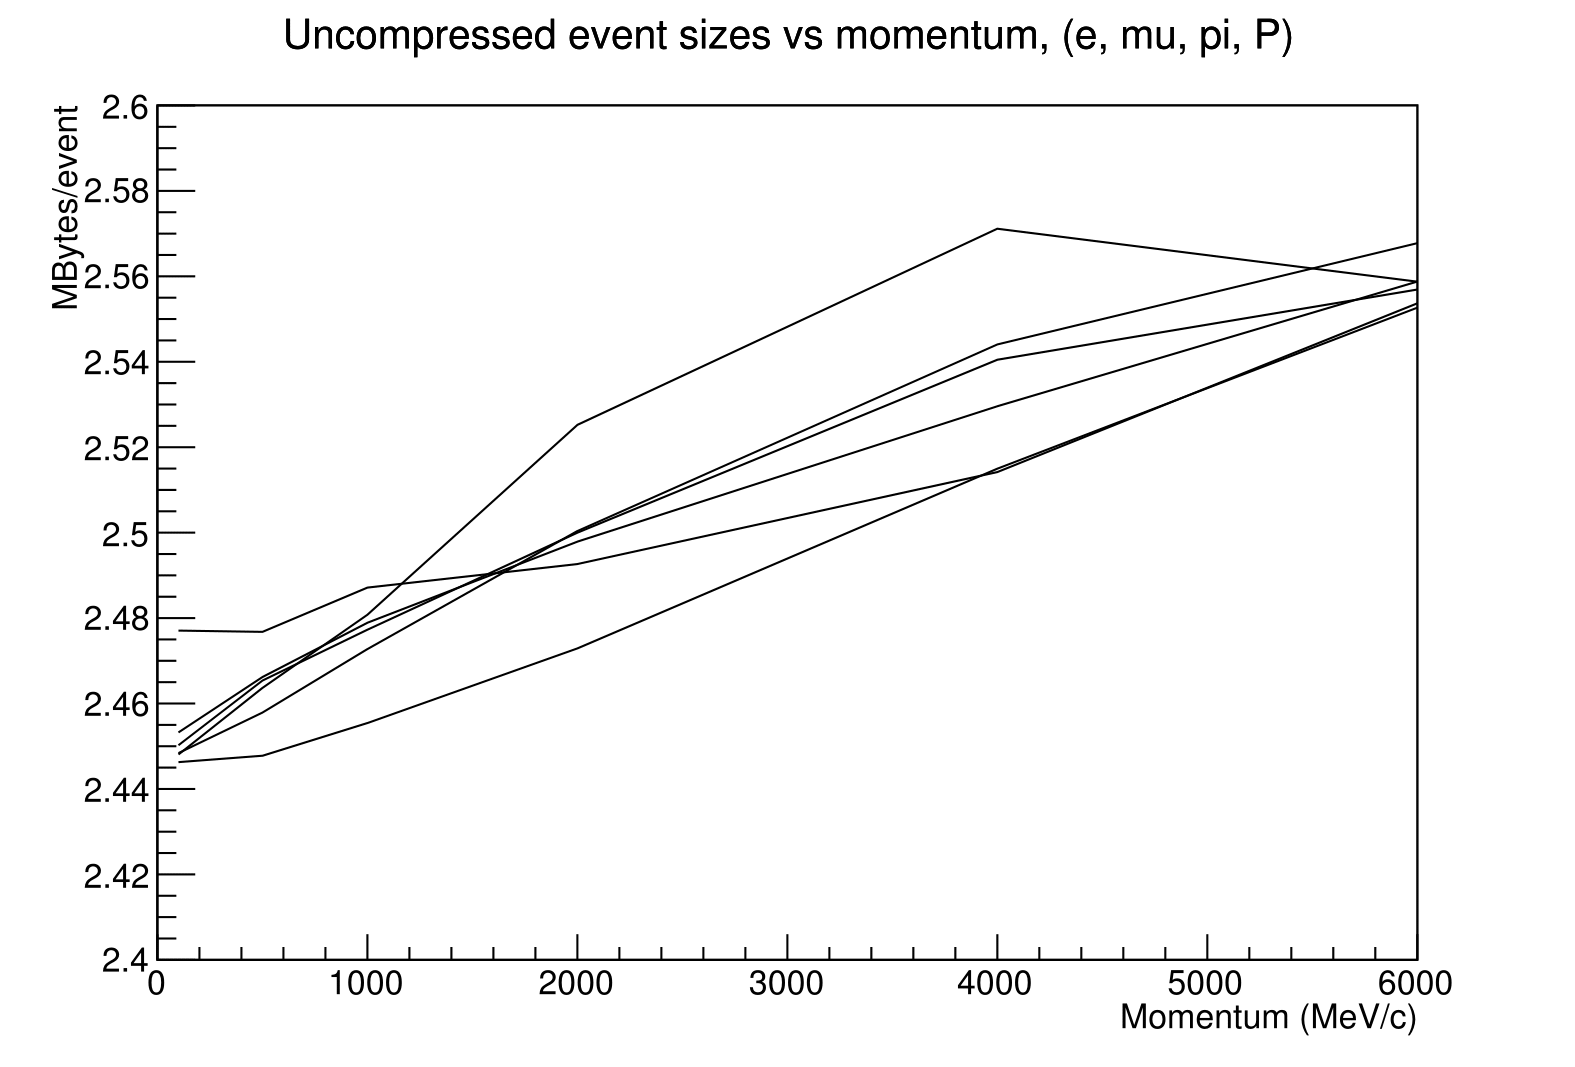
\includegraphics[width=0.6\textwidth]{btot.png}
	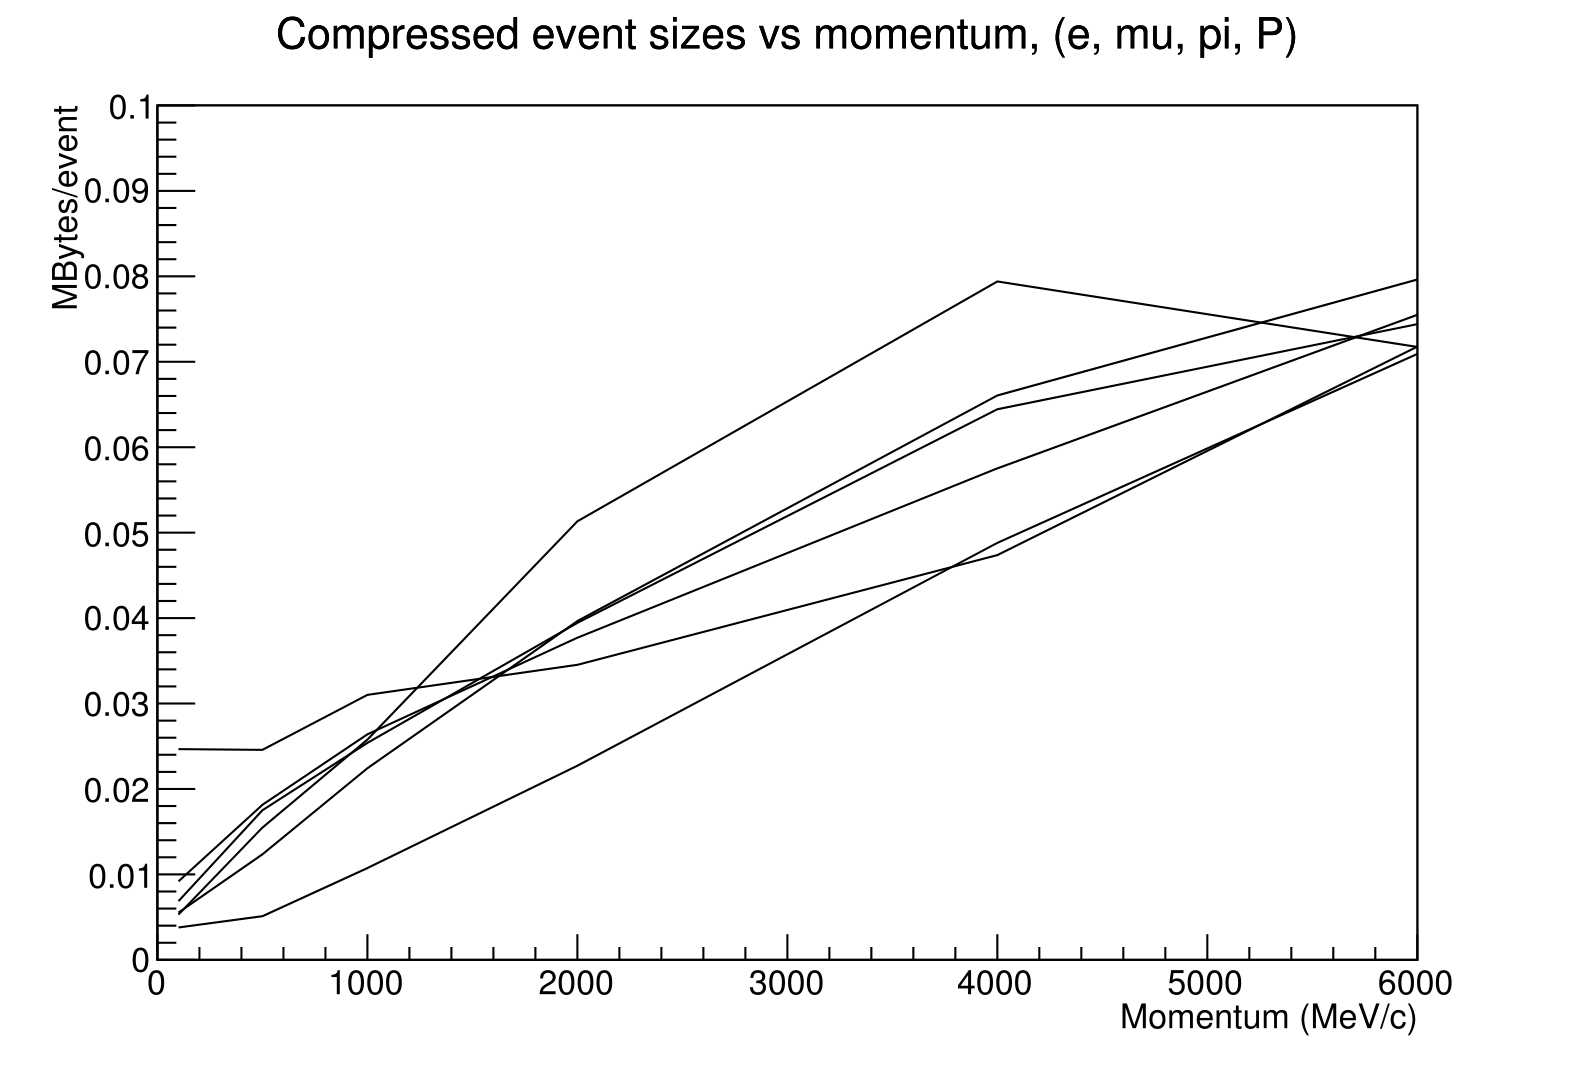
\includegraphics[width=0.6\textwidth]{bzip.png}
	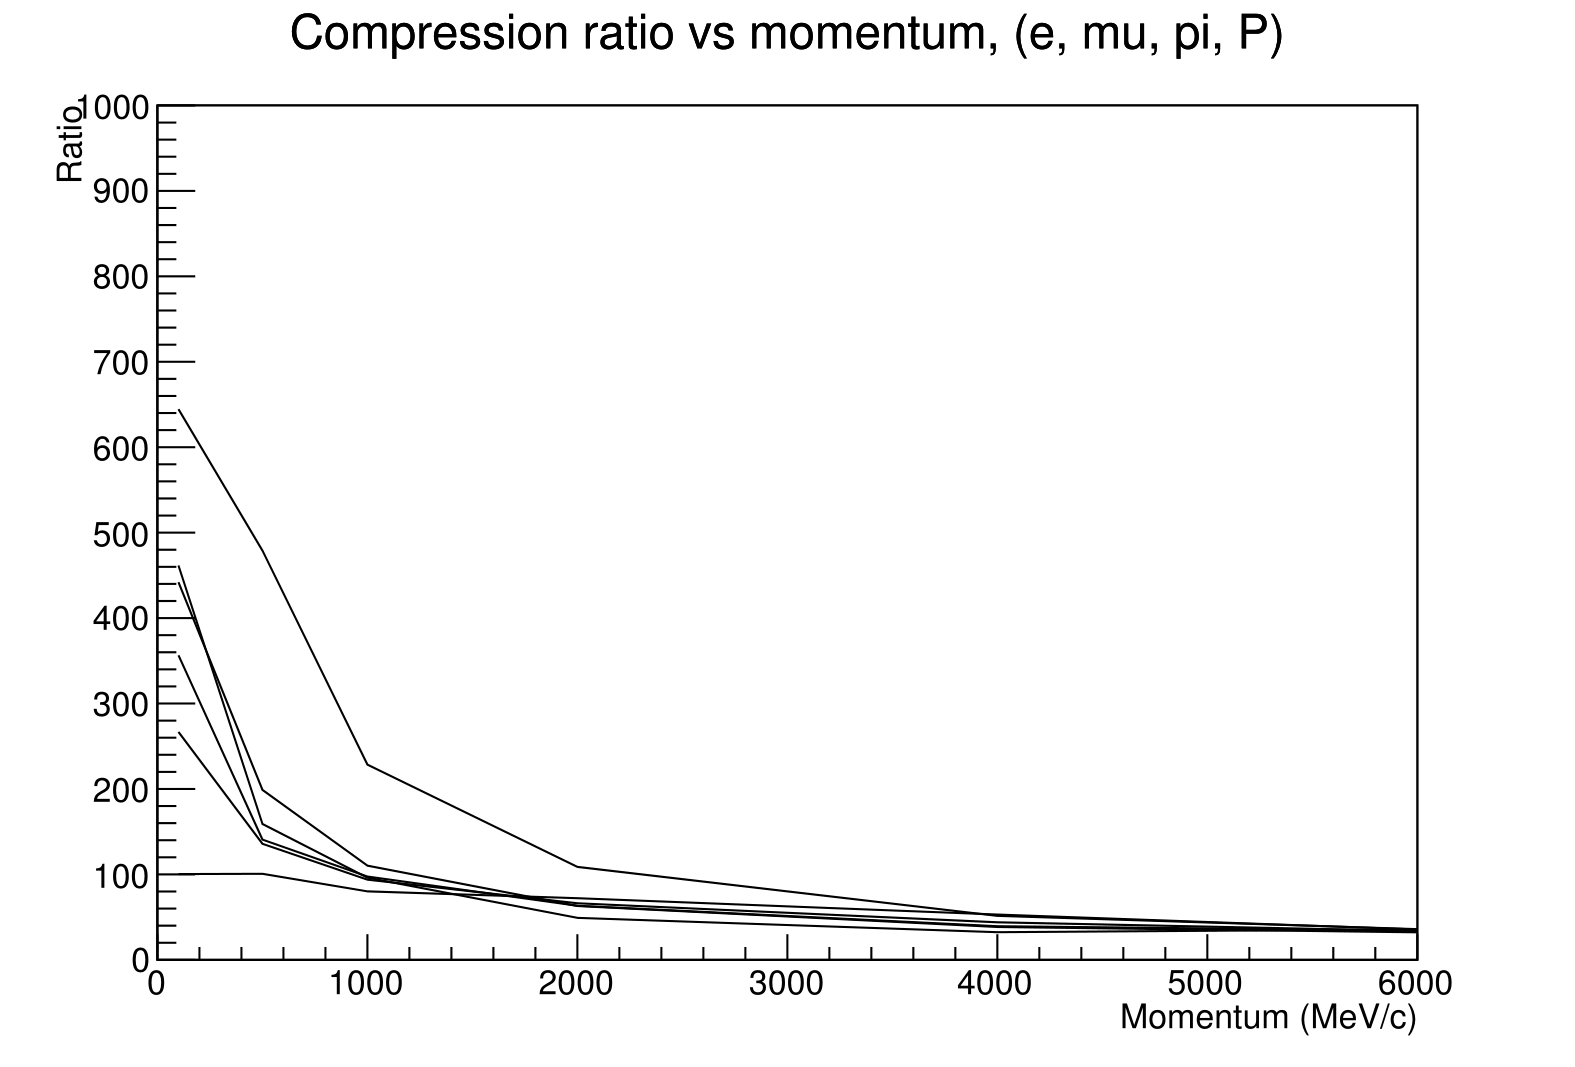
\includegraphics[width=0.6\textwidth]{brat.png}
	\caption{Estimation of DUNE zero-suppressed event sizes for different particles and momenta before (left) and after (center)  compression and their ratios (right).}
	\label{fig:data-compression}
\end{figure}
In order to estimate the effects of compression, specific particle types and energies were simulated using LArSoft.
The initial kinematics for the simulated samples covered a matrix of
particles ($e$, $\mu$, $\tau$, $\pi^+$, $\pi^-$, $\pi^0$ and proton) and momenta
(100\,MeV to 6\,GeV). The uncompressed and compressed sizes are summarized in Fig.~\ref{fig:data-compression}.

This exercise discovered a few types of inefficiencies in the design of data structures
currently used, which is unsurprising given that the DUNE software is undergoing active development
and not every optimization could be done until now. In one example, the bulk of the
compressed data written by LArSoft is actually made up channel ID
numbers providing a data inflation of about a factor of 10.
For uncompressed data this added about 50\%.
There are also additional data elements which are likely superfluous or
repeated more frequently than is likely to be required.
For example, in some types of the LArSoft output, even though zero suppression is applied, every
channel has an associated a pedestal and a sigma. There are other bits of superfluous data, but
they are not included in Fig.~\ref{fig:data-compression}. From the data presented in these
plots, the change in uncompressed event size is only a minor function of event momenta and
particle types. This is likely to be due to LArSoft saving additional overhead for all
channels, even those that have been fully zero-suppressed.

The simulation used to create these estimated included a detector module with
300,000 wires. The fact that the channel count in the full reference detector is
some 5 times larger will not change these estimates by a considerable margin
since it is assumed that DAQ/online systems will be capable of
not only of zero-suppression and compression, but also of suppression
of diffuse radiological backgrounds (see~\ref{sec:daq-assumptions}).
In other words, under normal conditions a cosmic $\mu$ or a beam
neutrino interaction will result in a localized ionization pattern (which
however may include long tracks) and the resulting data will not
scale linearly with the total channel count of the detector (which
sill still be effectively ``empty'' after suppression of $^{39}$Ar
background).

We then select the uncompressed event size to be 2.5\,MB and
the compressed event size of 0.2\,MB based
on data presented in Fig.~\ref{fig:data-compression} and
introducing a ``safety factor'' of 2 since the exact performance
of the data structures used in the final detactor cannot be precisely predicted at this time.

\subsubsection{High-threshold data volume summary}
\label{sec:fd-data-volume-summary}
Taking into account arguments presented above, and uncertainties of up to factor of 3 in the Zero Suppression
performance to be realized in the final system (see~\ref{sec:zs-data}), we summarize data volume estimate for
the high energy domain in Table~\ref{tab:fd-data-volume-summary}.
\begin{table}[ht!]
\centering
\begin{tabular}{| p{1.2in} | p{0.95in} | p{0.75in} | p{1in} | p{0.9in} |}		\hline	
Source & Event Rate & Event Size & Data Rate & Volume/year \\ \hline
cosmic-$\mu$ & 0.259Hz & 0.6\,MB & 155.4\,kB/s & 4.8\,TB \\ \hline
beam-$\nu$ & 8770 year$^{-1}$ & 0.6\,MB & 0.17 kB/s & 5.3\,GB \\
\hline
\end{tabular}
\caption{Summary of revised data rate and volume estimations corresponding to (HE) threshold.}
\label{tab:fd-data-volume-summary}
\end{table}



\subsection{The Near Detector Data}
\label{sec:nds-event-rates}
At the time of writing, there are many parameters of the NDS (see~\ref{sec:nds-params})
that are yet to be well defined. One set of parameters being considered at the time of writing is presented in
Table~\ref{tab:nds-params}. Table~\ref{tab:nds-event-rates} summarizes current estimates of the event rates
in the ND systems from various sources.

\begin{table}[ht!]
\centering
\begin{tabular}{| p{0.8in} | p{0.8in} |}		\hline		
\textbf{Source} & \textbf{Rate} (Hz)\\ \hline
Beam-$\nu$ & 40.2 \\ \hline
Rock & 10.0 \\ \hline
Cosmic & 0.04 \\ \hline
Total & 50.2 \\ \hline
\end{tabular}
\caption{Summary of combined DUNE Near Detector system event rate estimations.}
\label{tab:nds-event-rates}
\end{table}
\noindent
The projected data rate from the NDS is based on these event rates and occupancy estimated in preliminary Monte Carlo Studies,
and estimated number of samples to be read out per trigger ($\sim$4000). Preliminary size of each sample is 5B, resulting in an estimate
of $O(1)$\,MB per second data rate from the NDS. More information will
be added to these estimates as the R\&D in this area progresses.
\fxnote{More development needed here and more information from the ND people}

\newpage
\section{Far Detector Data Acquisition and Monitoring}
\label{sec:daq}

\subsection{Overview}

The scope of the DAQ and Monitoring work area includes the design, procurement, fabrication, testing, delivery and installation.
It is required to:
\begin{itemize}
\item collect data with a very high uptime (the goal is $>99\%$)

\item collect beam neutrino, atmospheric neutrino and proton  decay candidate events (generally all interactions
with total energy deposition above about 100\,MeV) with high resolution and virtually no dead-time.
%(smart or no zero-suppression) with

\item have the capability to collect interactions with total energy  below $100$\,MeV with some
 low amount of zero-suppression loss.

\item have the ability to trigger at the time of the beam pulses,  irrespective of how little energy is deposited in the detector.

\item provide the Supernova Burst trigger, i.e. collect data with the most favorable zero-suppression possible over a  period of >10\,s
and identify the characteristic signature of such event.

\item assemble data from sub-detectors into a unified  event for offline analysis.
\item provide access to the shift operator and others to control and   monitor the data collection and detector status, view online
  histograms and monitor (and provide for offline use) historical  status of measured detector parameters. 

\end{itemize}
% -mxp- edited out the no-ZS clause for the moment, on 12/20/2015  \fxnote{Need to reconsile the no-ZS stance here with ZS elsewhere}
\noindent
This section outlines a conceptual design intended to meet the required performance for the DAQ
for the DUNE far detector. 


\subsection{The DAQ Architecture}
\label{sec:daq-architecture}
To reduce downtime considerably (i.e. time periods when none of the DUNE modules are collecting data, which impacts supernova detection)
and to allow the DAQ technology in the different 10\,kt sections to be entirely different if desired, the DUNE DAQ employs a decoupled 
design. The synchronization, triggering, data collection and run-state in the different 10kt modules are completely independent in real time and
are only coupled by processes running asynchronously (in the same fashion as a batch queue) in the hour or so after data collection.
This allows one portion of the detector module to be restarted without interrupting
data collection in the others.

The layout of the DAQ is shown schematically in Fig.~\ref{fig:fddaqblock}.  To collect full detail of the
important high-energy events (detection of all those with energy deposition of 100\,MeV and above with virtually no dead time),
while avoiding tricky communication to flag neighboring channels to those that have large hits, a model is used
in which the digitised data are collected twice from the initial data
storage that is associatated with each peice of hardware. 

%%%%%%%%%%%%%%%%%%%%%%%%%%%%%%%%%%%%%%
% GB - I can't think of anything better, unless we expand this section
% a lot, which whould give it too much emphasis.  Ideally we DO want
% to flag neighbouring channels to those with big hits, but it is
% difficult because it would entail a big complicated network of
% comunications between all the boards which is very tricky.
%\fixme{Previous sentence not clear: you want to flag channels that have large hits and NOT flagneighboring channels?  What's the `tricky communication'?}

The first collection supplies a centralized software-based trigger farm continuously with
zero-suppressed information (a threshold on each channel detects hits above the noise level, also see \ref{sec:zs-data}).  
The second collection reads the full data at the times and in the regions %of interest that have been 
selected by the trigger. This is similar to the multi-level triggering in a collider experiment,
but with only one level of triggering. The software trigger farm also
records the continuous stream of zero-suppressed hits in an archival
ring buffer on disk to allow later analysis of supernova candidates.

\begin{figure}[h!]
	\centering
	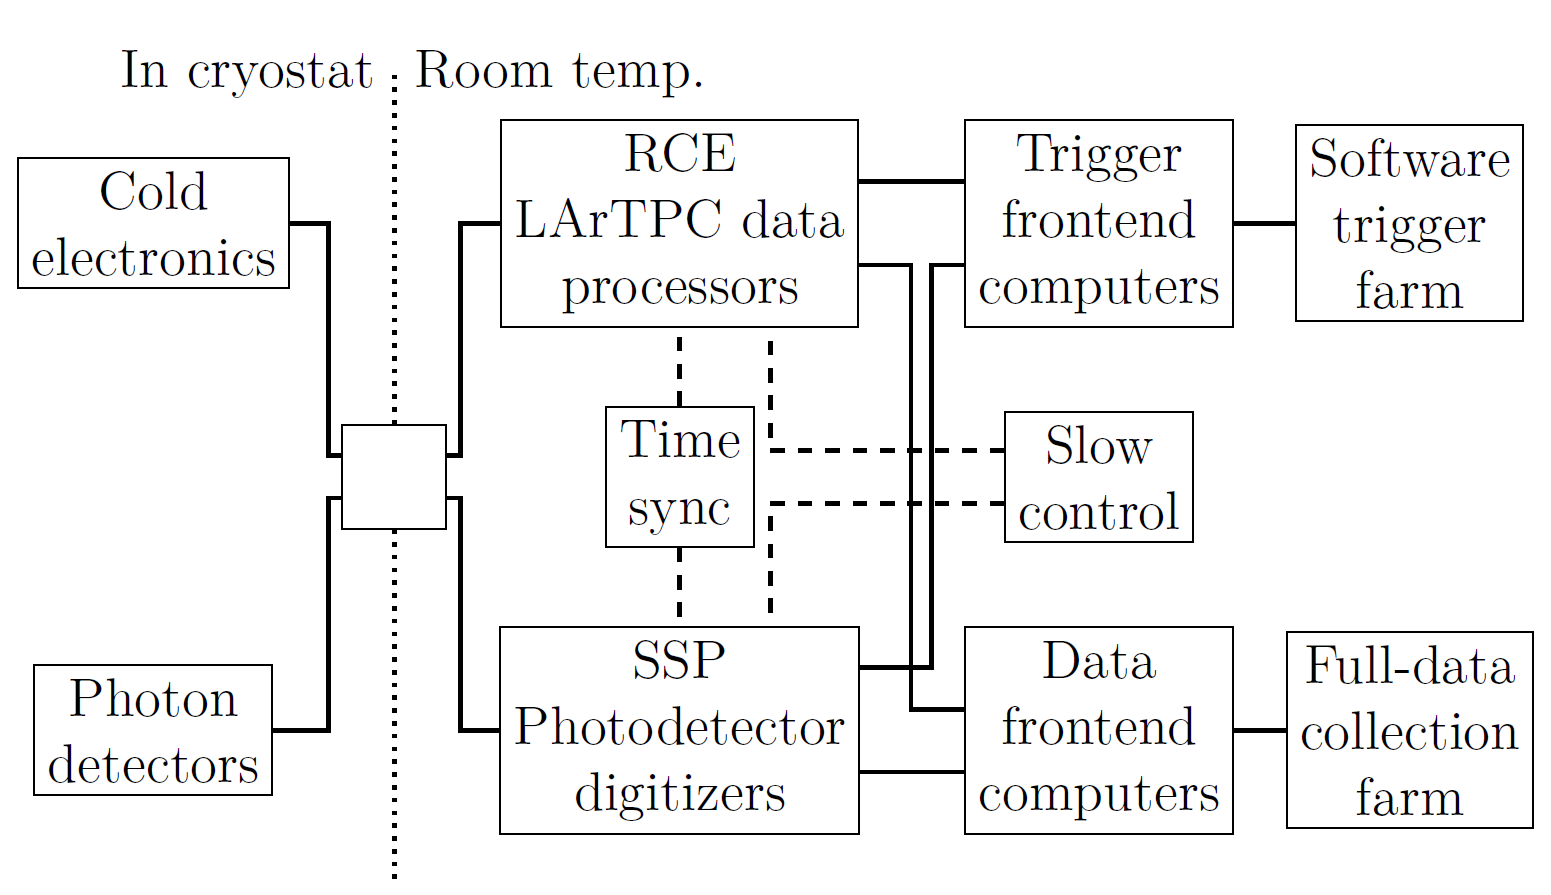
\includegraphics[width=0.8\textwidth]{daq-block-diagram.png}
	\caption{Block diagram layout of the main components of the DAQ subsystem.}
	\label{fig:fddaqblock}
\end{figure}

\noindent
Such architecture also allows to fulfill the requirement for the nucleon decay detection set forth in the DUNE Conceptual Design Report,
which is ``The Far Detector DAQ must enable continuous recording of data, outside of any beam gate, and retain enough information from
the front end (including photon system) through the DAQ chain to enable a trigger on events of interest'' \cite{cdr_vol2}.

\subsection{Hardware and Software Components of the DAQ}
\subsubsection{LArTPC detector readout}
An important feature of the Far Detector LArTPC front-end electronics is its placement inside
the cryostat, i.e. in the environment  with characteristic temperature defined by the liquid argon.
The LArTPC signals are digitized ``in the cold'' in a continuous flash-ADC stream at 2\,MHz, (not zero-suppressed)
and serialized on 12,000 high-speed links per 10kt module that exit the cryostat.

The data are received by LArTPC data processors located outside of the called RCEs \cite{slac_rce_1} (Reconfigurable
Computing Elements) housed in industry-standard aTCA crates on COB (cluster-on-board)
motherboards that are designed at SLAC for a wide range of applications.  The RCEs are part of a
network of field programmable gate arrays (FPGAs) that buffer the full raw data,
zero-suppress it for passing to the trigger and accept requests for
data-fetching from the trigger.  The FPGAs in the RCEs are from the
Xilinx Zynq family and contain a full Linux processor system on the
chip.  They facilitate the high-speed data transfer from firmware into
DRAM memory that is accessible from Linux.  A fast data-transfer
network using the Ethernet protocol is used on the COBs and in the
aTCA crates to allow for development of more sophisticated zero-suppression algorithms
for improved supernova acquisition.

\subsubsection{Photon detector readout}

As described in~\ref{sec:pd}, the Photon Detector readout  is performed by the ``SSP'' module.
 The additional buffering required for the separate trigger and data collection paths
is implemented in the SSP frontend computers.

\subsubsection{Computer farm}
Both the LArTPC and photon detector data are
received in commodity Linux computers, with no deadtime, from where
the data are routed to the trigger and full-data collection farms of
computers.  Although the front-end computers are logically distinct as
shown in Figure~\ref{fig:fddaqblock}, one physical computer is
sufficient for all the processes for each rack of APA readout
electronics. 

\subsubsection{The \textit{artdaq} software toolkit}

The \textit{artdaq} toolkit developed at  Fermilab supplies the real-time
data collection functionality (buffering, matching event parts,
synchronization, inter-process communication, etc.) in a modern
design that facilitates the efficient use of multicore commodity
computers running on the Linux computer farms.  The multi-core
functionality is crucial in the high data-rate environment on DUNE.  
The detector-specific code is supplied by DUNE groups
%(this is centered in the UK),
along with detector-specific triggering.
% (also UK). 
The architecture
provided by \textit{artdaq} can be tailored for each experiment and is entirely
suitable for the ``collect-twice'' architecture envisioned for DUNE.

\subsubsection{Run Control and Slow Control software framework}

This framework manages the control, status display and status archival of the experiment,
and is based on the ICECube design.  This exploits a combination of readily available, proven and
well-supported packages (e.g. zeroMQ for message passing, Django for web-framework etc) 
to give the shift operator a unified view of the status
of the running experiment, and views of the monitoring data including
customized views and historical views.  The database of slow-control
measurements is exported to the host lab to give access for offline
programs.

\subsubsection{Timing system}
To acomplish the software-based data acquisition in DUNE without dead time, it is
necessary to synchronize the clock across all readout boards.  This is accomplished
in two stages, the main cavern-wide distribution uses the design from the NO$\nu$A
experiment which distributes a 64MHz clock, synchronization pulses and
cable-delay correction on RJ45 cables.  The overall clock is
synchronized using a GPS receiver and transferred from the surface
over optical fiber.  The synchronization is transferred from the COBs
to the electronics in the cryostat over the same cabling as provides
the data links.

\subsubsection{Calibration system}
\label{sec:daq-calibrations}

At the time of writing, the calibration system is in the R\&D stage and its design will
evolve as the experiment is being built. Very roughly, there will be three stages:
\begin{enumerate}

\item Pedestal and charge-injection pulser events are used to calibrate and
remove drifting of the individual electronic channel responses.

\item External UV lasers are directed into the cryostat through glass-tube
ports, and swivelling mirrors select the trajectories of the beams
through the cryostat to provide calibration of the field
non-uniformities and attenuation.

\item Cosmic-ray muons are used for the determination of the energy scale and for calibration
cross-checks.

\end{enumerate}



\subsection{The DAQ Time Sequence}
\begin{figure}[h!]
	\centering
	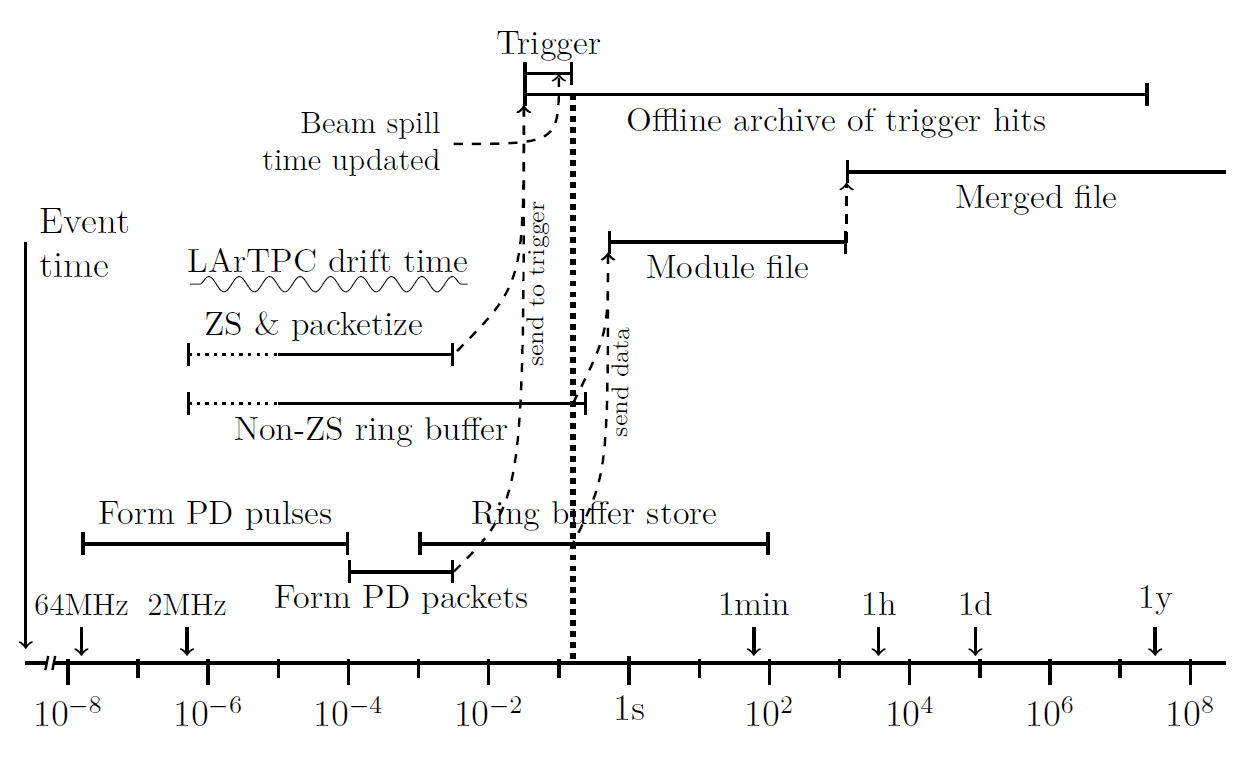
\includegraphics[width=0.8\textwidth]{daq-steps.png}
	\caption{Main DAQ steps displayed relative to the event time.}
	\label{fig:fddaqtime}
\end{figure}
\noindent
The time sequence, trigger deadlines and buffering of the readout are all
shown in Fig.~\ref{fig:fddaqtime}.  This figure shows time in the
horizontal direction on a logarithmic scale to indicate how long after
the particles appear in the detector each process can start and must
finish.  There is one level of triggering, with a trigger deadline
(latest time a trigger decision can arrive) of
0.16\,s after the event has occurred, indicated by the vertical dotted
line.  This is long enough that in 99\% of the cases, a message will
arrive from the Fermilab site to update the predicted time of a
neutrino spill with the actual time in order that the detector can be
triggered independently of any signals in the detector.  This approach
has been used succesfully in MINOS experiment for many years.  

As shown in Fig.~\ref{fig:fddaqtime}, prior to the trigger time and
independently in each detector module, the detector readout assembles
packets of data corresponding to fixed time intervals and sends them
to the trigger event builders.  Both the LArTPC readout and the SSP
readout (\ref{sec:pd}) send zero-suppressed data, suitable for triggering, to a set
of event-builder processes that run in parallel, each accepting all
the data from the entire 10kt module for a specific time interval and
performing trigger algorithms on them.  All time intervals are
processed so that the trigger has no dead time.  The data from the LArTPC and SSP
are also stored in ring buffers to await collection after an
affirmative trigger decision --- in the case of the LArTPC, this data
is not zero suppressed.  The data are built into events in a ``10kt-module
file'' that is written to disk.  About an hour later, an offline process merges
the data from the separate 10-kt module files and archives them at the host lab.

To maximize data collection for a supernova, the continuous
zero-suppressed trigger data is kept in a large buffer area on disk.
Ways to collect data that are cropped more gently than the zero-suppressed 
data stream during the extended period of a supernova are
under study: the non-zero-suppressed ring buffers on the current
design of RCEs are sufficient for 0.4\,s of buffering; the trigger farm can send
instructions in the trigger messages to manage storage of data in
these buffers during a supernova. Two possible extensions are

\begin{itemize}
\item extend the buffer memory , either on the RCEs or elsewhere in the aTCA crate

\item use the powerful intercommunications between RCEs to cause neighboring
channels to be kept around the time of a potential supernova event candidate

\end{itemize}

%\begin{cdrtable}[Estimated data rates]{lcc}{daqrefrates}{Estimated data  rates in the DAQ system}  %The third argument (reads {cc}) can use c, l, r or p{some length} % but please do %not include lines like “|c|l|l|”. It CAN look like {cll} or {llp{3cm}}, for instance.
%Process & Rate (kHz/APA) & Data rate (MBytes/s) \\ \toprowrule
%Generic 2.3\,ms interval & 0.43 & 6,000\\ \colhline
%Cosmic ray muons (4850L) & $6\times 10^{-7}$ & $1\times 10^{-5}$ \\ \colhline
%Radioactivity & $\sim 64$ & 1.9 \\ \colhline
%Electronics noise (not common mode) & $\sim 1$ & 0.03 \\
%\end{cdrtable}

%At the 4850L, the data rate in the trigger is dominated by
%radioactivity from $^{39}$Ar and $^{85}$Kr.  The cosmic-rays that
%occur about once per minute are the major source of events that should
%be collected on the data stream; the physics beam events, atmospheric
%netrinos and other candidate contained events are included in this data budget.  
%Table~\ref{tab:daqrefrates}) gives estimates of the
%rate of occurence of these events and the expected ``steady-state'' data rate
%(after the derandomisation provided by the buffering in the front-end
%computers).
\noindent
The requirements for handling radiological and other backgrounds (e.g. $^{39}$Ar decays as described
in~\ref{sec:ar39decays}) are met in this conceptual design by the very high throughput provided by modern
off-the-shelf components  and the parallelism provided by \textit{artdaq}, which makes the design extendable to avoid bottolenecks.  The triggering
allows the zero-suppression to be tuned to optimise for the final
level of noise, while retaining the maximum level of information for
the important physics events.

%This DAQ design is being prototyped for the 35t tests in 2015, with
%two COBs (containing 16 RCEs) and eight SSPs.  The \textit{artdaq} software
%toolkit is being used to implement the readout, event-building and
%triggering, although we are not implementing the ``collect-twice''
%model for the 35t.



\newpage
\section{Near Detector Data Acquisition and Monitoring}
\label{sec:daq-nd}

\subsection{Overview}
The Near Detector System (NDS) Data Acquisition system (NDS-DAQ)
collects raw data from each NDS individual DAQ, issues
triggers, adds precision timing data from a global positioning system
(GPS), and builds events.  The NDS-DAQ is made up of three parts, as
shown in the block diagram of Figure~\ref{fig:nds-daq-block}, a master DAQ
and one each for the near neutrino detector (NND, which is the FGT)
and the BLM systems. The names for these are, respectively, NDS-MDAQ,
NND-DAQ and BLM-DAQ.

\begin{figure}[h!]
\centering
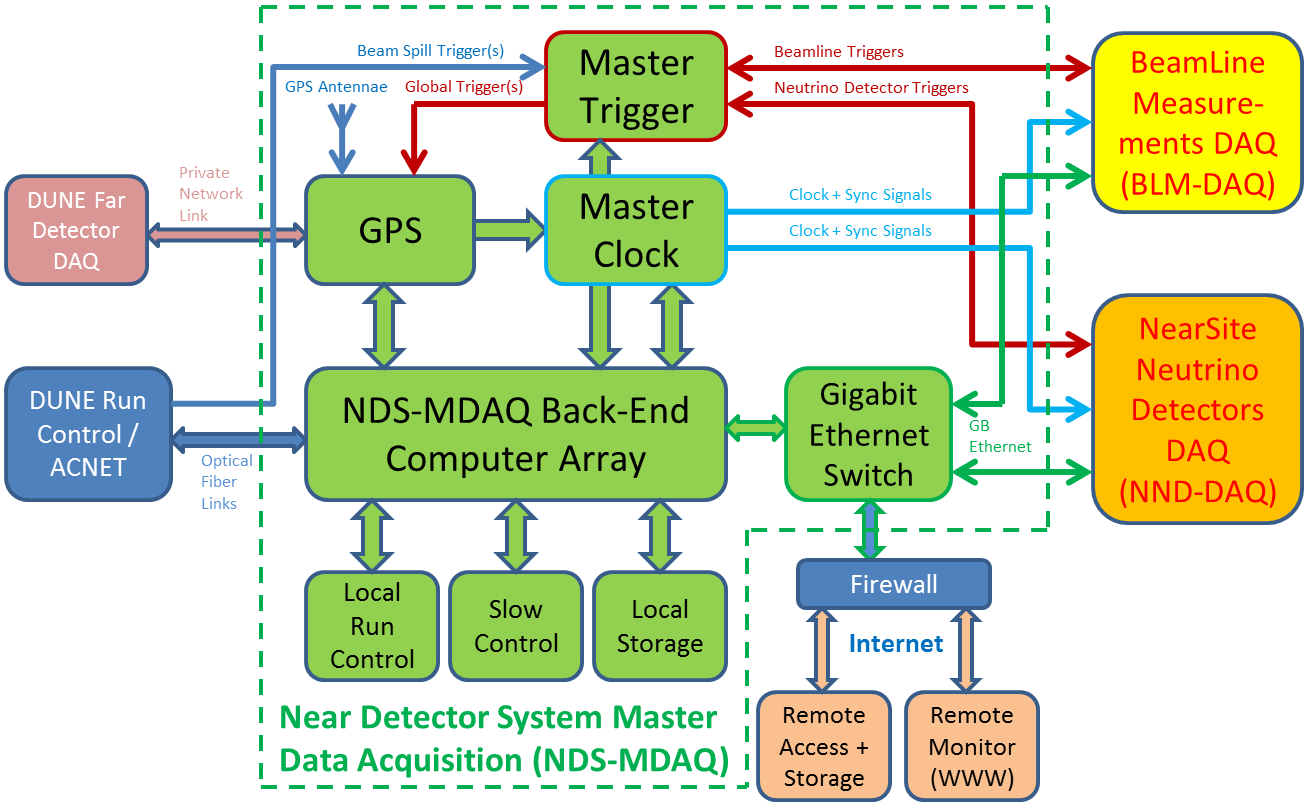
\includegraphics[width=0.8\textwidth]{daq-nd-block-diagram.png}
\caption{Near Detector System DAQ block diagram.}
\label{fig:nds-daq-block}
\end{figure}
%: The NDS-DAQ consists of the NDS Master
%DAQ (green blocks), the Beamline Measurement DAQ (yellow summary block) and the Near Neutrino
%Detectors DAQ (orange summary block). The NDS-DAQ connects to other portions of DUNE and
%LBNF, shown here in other colors (blue, light red, tan)


\subsection{NDS Master DAQ} 
\label{cdrsec:nd-master-daq}

The NDS Master DAQ (NDS-MDAQ) is designed to provide a high-level user
interface for local run control and data taking, as well as for secure
remote control and monitoring.  It will serve as the primary interface
to the NND-DAQ and BLM-DAQ and will include the following:
\begin{itemize}
\item slow-control system 
\item online data and DAQ performance monitoring  
\item raw data collection
\item building of events
\item data storage.   
\end{itemize}
The NDS-MDAQ includes hardware two-way triggering for both the NND-DAQ
and BLM-DAQ, and GPS hardware for precision time-stamping and global
clock synchronization.  The design is currently based on a channel
count estimate of approximately 433,000 from the near neutrino
detector and additional $\sim$1,000 from the beamline detectors.  Custom
electronic components for the NDS-DAQ are based on existing custom
designs from other experiments, e.g. T2K and ATLAS, and implement
commercial components for the trigger modules, clock and timing
synchronization, GPS and environmental monitoring.

\subsection{Near Neutrino Detector DAQ} 
\label{cdrsec:nd:nnd:daq}


The Near Neutrino Detector Data Acquisition system (NND-DAQ) collects
raw data from the DAQ in each NND subdetector and connects to the NDS
Master DAQ via Gigabit Ethernet. A block diagram of the NND-DAQ is
shown in Figure~\ref{fig:nds-daq-block}. 

\begin{figure}[h!]
\centering
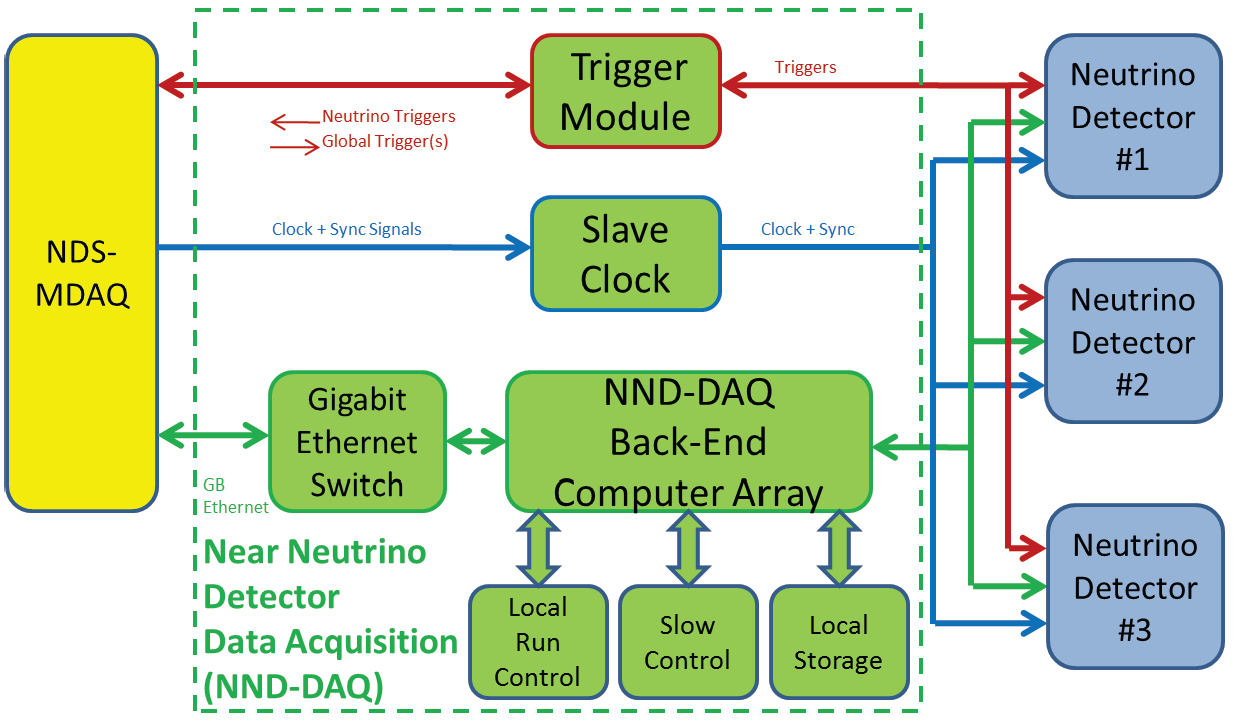
\includegraphics[width=0.8\textwidth]{daq-nnd-block-diagram.png}
\caption{Near Neutrino Detector DAQ.}
\label{fig:nds-daq-block}
\end{figure}

The NND-DAQ will mainly consist of a scalable back-end computer array,
interconnected to the individual subdetector DAQs via Gigabit
Ethernet and specialized electronics modules for trigger processing
and clock synchronization. It interfaces to the NDS-MDAQ for run
control and data collection. The NND-DAQ will also have its own local
run-control setup, consisting of a number of desktop workstations to
allow independent local runs that include NND subdetectors only; this
is useful during detector commissioning, calibration runs, stand-alone
cosmic runs, or other runs where the beam is stopped or not needed.

The quantity of computers required for the NND-DAQ back-end system is
highly dependent on the number of channels and expected data rates of
the individual neutrino detectors.  One back-end computer should be
able to handle approximately 3,000 channels for sustainable and
continuous runs. Assuming a total of 433,000 channels for all NND
subdetectors combined, about 150 back-end computers would be needed.

Trigger signals from each subdetector will be collected and
pre-processed by a trigger electronics module, similar in design to
the NDS trigger or master-clock modules of the NDS-MDAQ
design. Depending on the run mode, this module could feed local
trigger decisions to the detector DAQs for data collection, or it
could forward NDS triggers from the NDS-MDAQ or higher levels to the
NND subdetector DAQs.  A slave-clock electronics module, similar to
the master-clock module in the NDS-MDAQ, distributes clock- and
time-synchronization signals from the NDS-MDAQ to all NND
subdetectors.

\subsection{Beamline Measurements DAQ}

The Beamline Measurements DAQ (BLM-DAQ) will mainly consist of a scalable back-end computer array,
interconnected to the individual beamline measurement detector DAQs
via Gigabit Ethernet and specialized electronics modules for trigger
processing and clock synchronization. It interfaces to the NDS-MDAQ
for run control and data collection. It will also have its own local
run-control setup, consisting of a number of desktop workstations to
allow independent local runs that include beamline measurement
detectors only; this is useful during detector commissioning,
calibration runs, stand-alone cosmic runs or other runs where the beam
is stopped or not needed.


\subsection{NDS Computing}
\label{sec:nd-gdaq-global-computing}

The computing system encompasses two major activities: online
computing with required slow-control systems, and offline computing
for data analysis and event simulation.  The computing components are
based on currently available commercial computing and gigabit
networking technology, which is likely to improve over the next years
without driving costs up for the final design.

\fxnote{Work in progress!}


%%%----- THE COMPUTING MODEL. new layout - DUNE kept here, prototypes moved to the Appendix -----
\newpage
\section{DUNE Computing Model}
\label{sec:computing_model}

\subsection{Introduction}
The main purpose of the Computing Model is to guide the creation of DUNE computing fabric, spanning
hardware, middleware and various software components. Such fabric would give to all members of the DUNE
Collaboration unhindered access -- regardless of their location -- to reconstructed data for analysis, to various monitoring facilities,
to raw data for calibration and any other activities as required by the scientific objectives of the experiment. To meet these goals,
and in fulfillment of the data access requirements (\ref{sec:rules-of-access-to-data})
the model presented here has at  its core distributed data management and Grid and Cloud Computing concepts.

\subsection{Summary of raw data rate and volume estimates}
Rate and volume of the data to be produced by DUNE detector systems are the major driver determining the parameters
of the DUNE computing model. These characteristics  have been presented and discussed in detail in Sec.~\ref{sec:fd-data-overview}.

At the time of writing estimations for the Far Detector data are better understood compared to other DUNE subsystems,
due to better developed geometry and parameters of the LArTPC, technology and configuration choices, and considerations
presented in subsections~\ref{sec:daq-assumptions},~\ref{sec:zs-data} and \ref{sec:data-compression}.

A distinguishing characteristic of the data flow in DUNE Far Detector is a significant data reduction factor to be achieved
in the Far Detector DAQ, as evidenced by the numbers presented in Tables~\ref{tab:full-stream-volume} and \ref{tab:zs-volume}.
The key assumption in this is the capability of DAQ to distinguish low energy signals  due to $^{39}$Ar decays spread
across the volume of the detector from more interesting physics phenomena (see~\ref{sec:ar39decays}).
This and similar capabilities will be provided
by deploying appropriate algorithms on the DAQ RCE and online farm utilizing about a hundred computers (estimated).
Estimates of volume of data due to high-energy interaction (cosmic $\mu$ and beam neutrinos) are presented in
Table~\ref{tab:fd-data-volume-summary} (page \pageref{tab:fd-data-volume-summary}) and are quite modest.

Processing required to identify candidate SNB and nucleon decay events will also be handled by the DAQ system and its online farm.
As discussed in subsection \ref{sec:snb-data}, once a SNB trigger condition has been established, the data must
be recorded without zero suppression in order to capture the characteristically low energy and scattered ionization
clusters in the detector volume as expected in a supernova burst event. As shown in Table~\ref{tab:zs-volume} (page~\pageref{tab:zs-volume}),
the resulting volume of data is significant and is currently estimated as just over half a PB annually, given the premise of accepting roughly
12 false positives per year. While the main goal of the SNB trigger is to provide a close to real-time Supernova Burst alert, the data
flagged by DAQ as candidate should not be discarded as it can be used to better understand and improve online algorithms.

Identifying candidate nucleon decay events will also require algorithms that would set the trigger condition consistent
with signatures such as $p \rightarrow K^+\nu$. As shown in \ref{sec:pdk-data}, the volume of data due to such candidate
events is not expected to be appreciable compared to other sources.

The Near Detector is quite different from the Far Detector in all of its characteristics, and it includes a number of subdetectors
such as Fine-Grained Tracker, Electromagnetic Calorimeter and others (see~\ref{sec:nds-event-rates}). There are a few technology
options being conisdered and most parameters are still being finalized at the time of writing, so data estimates are very preliminary.
Current numbers result in annual volume from a few dozen to a hundred TB.

In summary, it is anticipated that under assumptions presented above the total volume of data in DUNE to be
committed to storage will be up to 1PB per year of data taking.

\subsection{Far Detector Data Handling}
\subsubsection{Conceptual Design of Data Flow}
A high-level conceptual diagram of the data flow in DUNE in presented in Fig.\ref{fig:DUNEdataflow}.
\begin{figure}[h!]
\centering
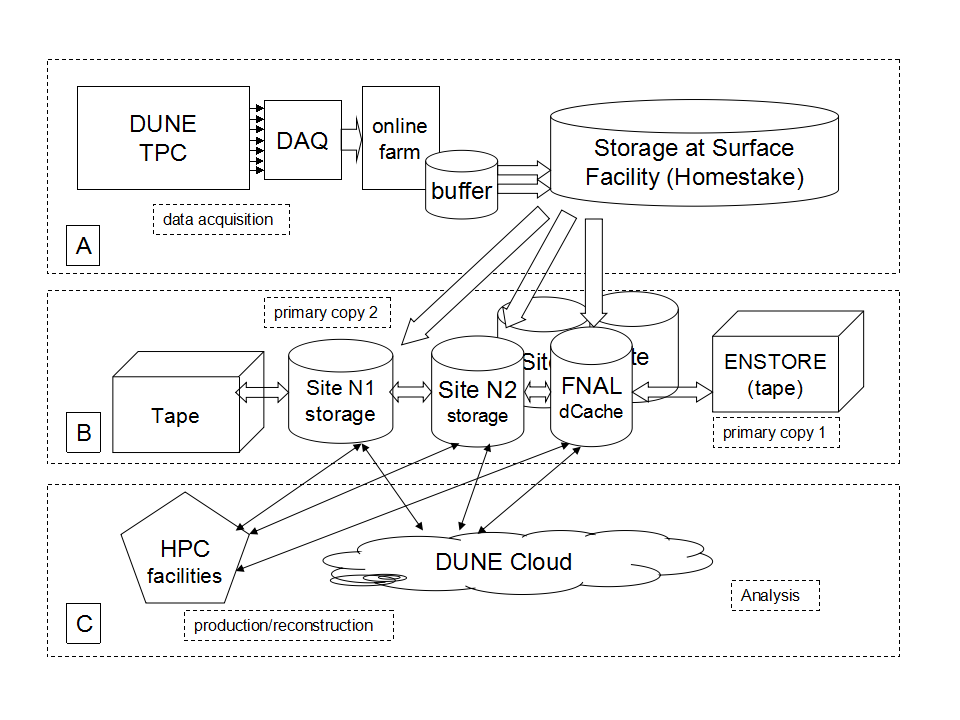
\includegraphics[width=\textwidth]{DUNEdataflow.png}
\caption{Conceptual Diagram of the Data Flow in DUNE.}
\label{fig:DUNEdataflow}
\end{figure}

\noindent
The top section of the diagram (labeled ``A'') represents systems and data flow at the Far Site.
The mid-section ``B'' depicts the DUNE data storage network. FNAL is the main data center
hosting tape storage for the primary copy of all data, as well as distributed disk (such as dCache).
It is expected that the Metadata system will also be deployed and operated at FNAL.
Additional Grid sites at participating institutions will have replicas of the data.
Replication of the data will be done as per requirements formulated in \ref{sec:req-raw-data-replication}.

\subsubsection{Data Buffering and Merging at the Far Site}
Data Acquisition systems will be located in the specially built rooms in the detector vicinity, i.e. deep in the cavern (commonly referred to as 4850L).
The undergound location is to be connected to surface by 96-strand fiber optic cable, but this does not imply that all strands will be
utilized at any given time. The scale of bandwidth of an individual fiber is 10gbps. It can be therefore expected that there will be ample headroom
for data transmission to the surface under a variety of scenarios.

There will be two layers of data buffering: a buffer in DAQ before the data is transmitted to the surface,
and at the surface facility before the data is transmitted to FNAL which is the primary storage site and the
keeper of the custodial copy of the data.

It is a common practice to provide buffer space for the experiment which is sufficient for intermediate storage of data
for one or maybe a few days in order to keep running even in case of network equipment outages. Given the estimates
presented above, the decisive factor for determining the buffer size will be the data scale of candidate SNB events since
they are likely to be read out at full-stream rate (with lax or no zero-suppression) (see Table~\ref{tab:zs-volume}). The
size of each buffer (the online farm and the surface facility as drawn in section ``A'' of Fig.\ref{fig:DUNEdataflow})
can therefore be estimated as $\sim$50\,TB.

 There are additional considerations due to the modular structure of the DUNE Far Detector
which is conceived as four individual TPC modules. In order have to have more flexibility and to minimize down time
and the number of potential single points of failure the DAQ will be segmented into four individual  systems each collecting
data from their respective module~(see \ref{sec:daq-architecture}). To ensure
consistency and simplicity of processing, it is desirable to merge the data streams coming from individual detectors' DAQ systems
at some point so that data is written to files contains readout for the full 4-module DUNE detector. The surface facility is the optimal location
for the merging to take place since it needs to be equipped with storage and networking equipment for buffering purposes in any scenario.

\subsection{Data Handling at the Near Site}
\fxnote{Just a placeholder at this point}
The Near Site is located within the boundaries of Fermilab and therefore it is easier to provide networking and other services for data handling.

\subsection{DUNE Data Management}
\subsubsection{Types of data}
Principal types of data in DUNE will include raw and processed data (see \ref{sec:req-data-definitions}),
the latter term also applying to Monte Carlo data.

\begin{figure}[h!]
\centering
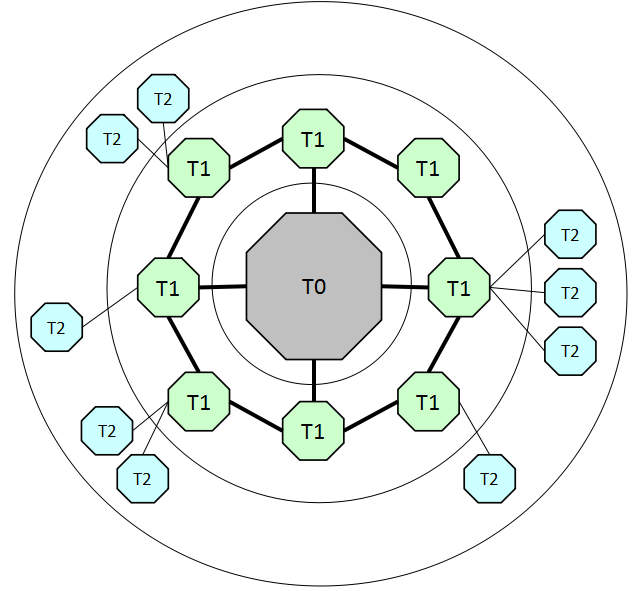
\includegraphics[width=0.6\textwidth]{monarc-model.png}
\caption{MONARC model of data distribution.}
\label{fig:monarc}
\end{figure}

\subsection{DUNE Analysis}
\subsubsection{Analysis Procedures and Data Flow}
\subsubsection{The Analysis Model}
\subsubsection{Distributed Analysis}

\subsection{Simulation}
\subsection{Calibration}


\newpage
\section{Resource Requirements}
\label{sec:resource-requirements}
\subsection{Overview}
The computing requirements of the DUNE experiment will evolve significantly between the time of writing
and comissioning of the full set of DUNE detector systems, for the following reasons:
\begin{itemize}
\item In short and medium term, active work will continue on DUNE prototypes, the ``35t prototype'' and protoDUNE
(see Sections~\ref{sec:35t} and \ref{sec:protodune} correspondingly).

\item Amount of R\&D work for the Near Detector is significant and it can be expected to ramp up as offline software
is being prototyped and extensive simulations will be required.

\item Investigation of optimal reconstruction methods for LArTPC is ongoing and far from complete. This means
that there will be fluctuating resource requirements (mainly CPU) for MC and reconstruction in the course of R\&D
as the algorithms are improved over the years.

\end{itemize}

\noindent
As many hardware and software components in DUNE are under active development,
and the final data model has not yet being created, there are necessarily large uncertainties in any resource requirement estimates
at the time of writing. It is however helpful to review current understanding of the general scale of number so as to provide some
guidance for DUNE resource need going forward.

In the following, ``best effort'' estimates are presented for resources required by the DUNE prototype work,  R\&D for the final DUNE
and ballpart values for what DUNE will need at the start of operations.

\subsection{Prototypes}
\subsubsection{35t}
Estimates for resource requirements for the 35t prototype are given in \ref{sec:35t-resource-requirements}.
In summary, the requirements are:
\begin{itemize}

\item Raw data on disk: $\sim$200\,TB

\item Disk space to support reconstruction: $\sim$400\,TB

\item Raw data committed to permanent tape storage: $\sim$100\,TB

\item MC data on disk: $\sim$100\,TB

\item CPU for reconstruction: $\sim4\times10^6$\,hours scaled to a ``standard'' Fermigrid node. This translates into $\sim$500 Worker Nodes
committed over a period of one year in order to get the data processed during that time.

\end{itemize}

\subsubsection{protoDUNE/NP04}
Eastimates of protoDUNE storage requirements are fiven in \ref{sec:protodune-zs} and \ref{sec:protodune-dataprocess}.
In summary, the requirements are:
\begin{itemize}

\item Raw data on disk: $\sim$500\,TB

\item Raw data committed to permanent tape storage: $\sim$500\,TB

\item Disk space for staging data at CERN before transmission: $\sim$100\,TB

\item Disk space at FNAL to support reconstruction: $\sim$1\,PB

\item MC data on disk: $\sim$100\,TB

\item CPU for reconstruction: $\sim$O(1000) Worker Nodes
committed over a period of one year in order to get the data processed during that time.

\end{itemize}

\subsection{DUNE}
\subsubsection{Data Volume and Storage Requirements}
Projections for various sources of data in DUNE and associated data volumes are given in
Table \ref{tab:summary-data-table} with comments provided in \ref{summary-annual-volume}.
Under assumptions given throughout Section \ref{sec:data-characteristics} and further detailed
in \ref{sec:data-rate-and-volume-estimates}, the synopsis is as follows:
\begin{itemize}

\item Recording Supernova Burst candidate events and preserving them for detaiedl analysis (which is necessary to take
full advantage of this unique capability in DUNE) will result in excess of $\sim$500\,TB of raw data annually, under the assumption
of 12 false positives per year. This is the largest single source of raw data in DUNE.

\item The Near Detector Systems are the second largest source of data with initial estimates of $\sim$100\,TB of raw data annualy.

\item Beam neutrino events, cosmic muon events and proton decay events combined are expected to produce
much less raw data than the leading sources, on the scale of  $\sim$5\,TB. Possible implications of this fact
are discussed in \ref{sec:implications-of-data-estimates} on page \pageref{sec:implications-of-data-estimates}.

\item MC data on disk: $\sim$40\,TB (annual).

\item Ratio of derived data to its source (whether its raw or MC) is assumed to be 2 based on extrapolation from other experiments.

\item An additional factor of 4 (the ``headroom'') is required to support reprocessing of the data (such as with improved calibrations etc)
and running two concurrent releases of DUNE software.

\end{itemize}

In summary, the estimated total storage requirement is estimated as $\sim$6\,PB (annual).

\subsubsection{CPU Requirements}
At the time of writing, Monte Carlo studies in DUNE result the following CPU utliziation pattern is observed according to Grid monitoring data:
\begin{itemize}

\item Far Detector MC: 6 campaign per year, 40\,k CPU*hrs each, total $\sim$240\,k\,CPU*hrs

\item Near Detector MC: 3 campaigns per year, 40\,k CPU*hrs each, total $\sim$120\,k\,CPU*hrs

\item Beam Simulations MC: 3 campaigns per year, 200\,k CPU*hrs each, total $\sim$600\,k\,CPU*hrs

\item MARS group MC: same scale as Beam Simulations, i.e. $\sim$600\,k\,CPU*hrs

\end{itemize}

\noindent
Total CPU budget for Monte Carlo is therefore approximately 1.5\,million CPU hours per year and this number
should be considered as basis for extrapolation going forward.

Situation with CPU power for reconstruction is much less clear due to the fact that this software has not yet been fully
developed at the time of writing and only rough prototypes exit. Judging from the event rates presented in this document,
reconstruction of the Near Detector will be a larger challenge than processing beam-$\nu$ and cosmic-$\mu$ events due
to relative complexity of the ND design and operating principle, and to an appreciable event rate
(see \ref{sec:fd-data-volume-summary} and \ref{sec:nds-event-rates}). Accepting the nominal ND event rate to be 50\,Hz,
and assuming a $\sim$1\,min per event reconstruction time purely as an order of magnitude estimate device, it can be estimated
that a few thousand Worker Nodes will need to be dedicated to the Near Detector data production, just to keep up with the nominal
data rate. This leads to a rough estimate of at least 30\,million\,CPU*hrs annually.

Reconstruction of the Supernova Burst candidate events presents more challenges with data logistics (due to the very large size
of the readout package) than with reconstruction since the total number of potential neutrinos in a single event is still O(10$^2$).
Currently the concusion is that the resulting CPU requirements will be substantially less than those for the Near Detector.






\newpage %%% prototypes are now in the Appendix
\newpage
\appendix
\section{Glossary, abbreviations and acronyms}
\label{sec:appendix-glossary}
\begin{description}
\item[AOD] Analysis Object Data
\item[APA] Anode Plane Assembly
\item[\textit{art}] Physics Software Framework developed at FNAL
\item[\textit{artdaq}] Data Acquisition Toolkit based on \textit{art}
\item[CASTOR] Tape storage system at CERN
\item[CDR] Conceptual Design Report
\item [COB] ``Cluster-On-Board'' (an element of the DAQ)
\item[CPA] Cathode Plane Assembly
\item[CIS] Continuous Integration System
\item[CVMFS] CERN Virtual Machine File System (network-based method of data delivery)
\item[DAQ] Data Acquisition
\item[Dataset] A collection of data, which may be a collection of files containing data of similar type (but not necessarily)
\item[DRAM] Dynamic random-access memory
\item[EOS] High-performance distributed disk storage system at CERN
\item[ESD] Event Summary Data
\item[FGT] Fine-Grained Tracker
\item[FPGA] Field Programmable Gate Array
\item[FS] Full Stream (data collected with zero threshold)
\item[HE] High-Energy threshold and data stream associated with it
\item[LArSoft] A software suite based on \textit{art}, focused on Liquid Argon TPC
\item[LArTPC] Liquid Argon TPC
\item[LBNF] Long-Baseline Neutrino Facility
\item[MC] Monte Carlo
\item [MONARC] Model Of Networked Analysis At Regional Centers
\item[NDS] Near Detector Systems
\item[Pandora] A software toolkit for event reconstruction
\item[PD] Photon Detector
\item[QA] Quality Assurance
\item[RCE] Reconfigurable Cluster Element
\item[Reprocessing] Processing the data more than once with same software release but different calibrations and possibly other differing parameters
\item[SAM] \textit{Sequential Access via Metadata} (a metadata and storage system at FNAL)
\item[SURF] Sanford Underground Research Facility
\item[SNB] Supernova Burst
\item[SiPM] Silicon Photo-Multiplier
\item[SSP] SiPM (Silicon Photomultiplier) Signal Processor
\item[Wirecell] A novel event reconstruction technique based on tomography
\item[WMS] Workload Management System
\item[ZS] Zero Suppression
\end{description}

%%%%%%%%%%%%%%%%%%%%%%%%%%%
\newpage
\section{Software and Computing Requirements}
\subsection{Overview}
\subsubsection{Purpose, Origin and Scope}

These \textit{Requirements} are in essence rules and guidelines for setting policies, putting in place practices (for example related to data handling)
and making technology choices in DUNE. They do not cover specific \textit{functional requirements} for the various physics tools software
or specific parameters (storage capacity, bandwidth, CPU hours etc) of DUNE computing, which are to be addressed in the Computing Model proper.
Instead, the focus of this section is on the foundations of the Software and Computing infrastructure, such as code management, Grid capability, data management etc.
An effort was made to maintain a relatively high-level view of the DUNE computing issues. In cases where it was impossible to establish concrete metrics or parameters
for a specific requirement, it is still listed as an item to be addressed in the future.
%, and to not go into smaller details which are more likely to change as the project moves forward, while still providing adequate basis for making informed decisions.

The \textit{Requirements} have been developed based in part on prior planning work done for the Long-Baseline Neutrino Experiment, which was a predecessor of DUNE.
They constitute one of principal components of the Computing Model. 


%Information necessary for the creation of these Requirements have been collected during a number of DUNE Software and Computing meetings, conference calls and extensive information %exchange via e-mail and other means. It is recognized that the Requirements themselves (and the Computing Model) may evolve with time, in order to correctly reflect the status of rapidly %evolving technologies and the DUNE organization itself. Such expectation is reinforced by actual experience of large scale HEP collaborations. We anticipate therefore that the requirements will %be revised roughly in the middle of the time period between their creation and the commissioning of the experiment, and help evolve the DUNE Computing model such that it continues to meet %the needs of the Collaboration.

%Certain  requirements need to be specified by a collaboration including the S\&C Organization and other software organizations in DUNE
%(i.e. the Physics Tools Group, the Online/DAQ groups etc). In these cases, the S\&C Organization will work with the appropriate group to insure
%that the requirement addresses the needs of all necessary organizations.  This includes interfacing with various DUNE Project groups in order
%to assure the seamless cooperation between the online and offline areas.

\subsubsection{Structure}

The \textit{Requirements} are organized as a set of categories reflecting major responsibilities of the DUNE Software working group.  Each category will generally
contain information including:

\begin{itemize}
\item \textbf{Description:} Description and scope of the category.
\item \textbf{Definitions:} If necessary, specific definitions of certain items are given.
\item \textbf{Issues:} Statement of issues that requirements in this particular category are expected to address.
\item \textbf{Requirements:} The requirements themselves, formatted as assertions.
\end{itemize}

Where necessary, each of these items may be placed in an individual subcategory to better reflect details and granularity of information being presented. A requirement section may be accompanied by one or more of the additional items:

\begin{itemize}
\item \textbf{Use cases}: Descriptions of any use cases that drive the choice for the requirement.
\item \textbf{Justifications}: Explanations as to why the requirement was chosen.
\item \textbf{Accepted risks}: Any known problems with the requirement which are considered acceptable.
\item \textbf{Alternatives}: Any alternatives that were considered with reasons for rejection.
\item \textbf{Deviations}: Recognized cases where deviations do not violate the intention.
\end{itemize}

In addition, in cases when it helps clarify the scope of a given  requirement, appropriate statements will be made as to what is \textbf{not} required in the context of a particular section.


%%% ++++++++++++++++++++++++++++++++++++++++++++++++++++++++++++++++++++++++++++++++++
\subsection{Data Requirements}
\label{sec:dunedata}

\subsubsection{Description}
This section contains the requirements related to handling a variety of data by the DUNE Collaboration. This includes data produced by DUNE primary detectors and monitoring systems, as well as derived (processed) datasets and other collections of data (and where necessary, the metadata associated with these items). Databases and related technologies will be covered separately in Section~\ref{sec:dunedb}.

The principal requirement for data distribution and access methods is that they need to support a coordinated and widely (indeed globally) distributed network of computing centers and research groups located at DUNE member institutions. This is closely related to Section~\ref{sec:dunedc} (Distributed Computing).
\fxnote{Make sure the referecnce to Dist Comp is correct}

Data Retention policies will aim to provide cost-effective and optimal schedule of data distribution, replication and retirement, in order to maximize
efficiencies in achieving the scientific objectives of DUNE. On a longer time scale, there is a need to put in place policies and procedures for data preservation.
The principal difference between retention and preservation is that the former concerns itself with optimizing ongoing analyses and other types of data processing,
whereas the latter addresses the long term storage and documenting and preserving methods of accessing these data (formats, algorithms, application code etc).


\subsubsection{Definitions}
\begin{itemize}
\item \textbf{Raw Data:} Data saved by a detector (far, near or prototype detector) DAQ or monitoring systems, and information from FNAL beam monitoring.

\item \textbf{Production Software:} the suite of software run to produce an official collaboration result. One example of such software is software used to produce data appearing in a publication. Such software is subject to strict version control, QA and validation, and is utilized in a managed fashion.

\item \textbf{Processed Data:} any data produced by production software (see above) for the collaboration as a whole or to satisfy the needs of working groups.  This includes simulations, data reduction/reconstruction, data skimming and inputs to final analyses. This type of data does not include data samples produced by individual users using software that has not been certified as production software by appropriate Working Groups, Production Managers and if needed by the S\&C Coordinators.

\item \textbf{File catalog:} a general term used to describe a system which performs a range of mapping functions, such as mapping of a Logical File Name (LFN) to one or more physical locations of the file in the distributed data management systems. This functionality is essential for locating physical copies of the data when needed, optimal matching of distributed data to available computing resources, storage accounting and various other aspects of distributed data management. File catalog may also incorporate functionality related to Metadata (see next item).

\item \textbf{Metadata:} data that describes other data.

\item \textbf{Dataset:} a collection of files (potentially in differing formats) and corresponding metadata (uniform across the set) that forms a coherent unit of data used in a computation, and is accounted for as such.
\end{itemize}

\subsubsection{Issues}
The following is a short list of issues that DUNE will need to address in its data handling:
\begin{itemize}
\item Data replication strategy for each major class of data needs to be created.

\item Data retention policies are an important tool to assure cost-effectiveness and overall efficiency of the  data infrastructure.

\item Long-term data preservation policies and procedures need to be properly planned.

\item General rules of access for DUNE collaborators, and for the general public need to be understood in order to assure efficiencies and compliance.

\item Data distribution and access methods will play a major role in resource availability and overall efficiency of resource utilization.

\item The file catalog is one of the central elements of many architectures for handling data, and its performance characteristics are of utmost importance.

\item File and dataset metadata: management of the large and heterogeneous volume of data in DUNE  (e.g. Monte Carlo samples, raw data, processed data in any stage of analysis or transformation etc) requires creation, storage and appropriate use of coherent metadata, which must allow identification, location and retrieval of collections of data necessary for specific purposes. It is crucial that the design of the metadata and any system for its utilization is such that it allows for truly distributed, highly scalable and symmetric strategy of data placement.

\item Loss of information contained in the file catalog and/or metadata system may have pernicious effects such as appearance of ``orphaned" or ``dark" data, i.e. data 
residing in storage that cannot be efficiently located and utilized by the Collaboration.

\item Data design and formats: having a consistent approach to data design and policies to maintain relevant standards and interfaces is crucial for efficient and reliable software development processes and operations of DUNE.

\item Raw data collected by DUNE  online systems (such as DAQ) will be stored (buffered) at a facility located close to the Far Detector, then transmitted to central mass storage via the network. Efficient interface for exchange of data between the online and offline systems needs to be established.

\end{itemize}

\subsubsection{DAQ Data Interface Requirements}
\begin{itemize}
\item Data formats, schemas and other crucial parameters pertaining to data recorded by DUNE  data acquisition systems shall 
be formulated and documented in close cooperation between the Software working group and Online Software/DAQ Group.

\item Handling of the data being recorded by DAQ systems shall become responsibility of the Software working group once such 
data is first deposited into a general purpose mass storage system, having passed necessary validation steps.

\end{itemize}

\subsubsection{Replication Requirements}
\textit{Raw data replication}

\begin{itemize}
\item Facilities storing official copies of the raw data shall possess adequate storage capacity, availability (i.e. minimal downtime), network connectivity and bandwidth as well as other relevant infrastructure characteristics to be determined by the Software working group.

\item The number of raw data replicas at any given time shall be sufficient to protect the raw data as a whole from data loss, by utilizing a variety of techniques such as redundancy inherent in replication, automated error detection, automated data repairs and others.


\item Raw data replicas shall not be required to reside in a single storage facility and may be divided in managed datasets distributed to a few designated DUNE computing centers chosen based on agreements with member institution and taking into account their infrastructure characteristics.

\item Latency of replication of raw data shall be within a 24 hour period, counting from arrival of new data to the initial storage location (buffer), and to the point where transmitted data is deposited in mass storage at the remote location, and validated and accounted for in the data handling system.

\item Any storage system or host selected for the official copy (replica) of the raw data shall employ storage technology with an expected loss of no more than one unit of data per million per year.

\end{itemize}

\textit{Processed data replication}

\begin{itemize}

\item The processed data shall be generated at, and distributed to DUNE computing facilities at participating institutions 
based on a combination of factors such as research interests of the corresponding working group operating at a particular location, 
resource availability and scheduling policies of the Workload Management System employed by DUNE.

\item The number of replicas of the processed data shall not be subject to a fixed minimum. 

\item The number and placement of replicas of the processed data shall be determined dynamically based on requests of a particular processing campaign, with priorities set by collective decisions of the Physics Working Groups and the Software working group.
\end{itemize}

\textit{General replication}

\begin{itemize}
\item Mechanisms shall be put in place to assert validity of the data being replicated and/or transmitted.

\item One mechanism for validating data replication shall be checksum controls.

\item Control of data placement, volume, status and other characteristics shall be available.
\end{itemize}

%%% --------------------------------------------------------------------
\subsubsection{Data Retention and Preservation Requirements}

\textit{Raw data retention}
\begin{itemize}
\item Raw data shall be stored at least for the duration of the experiment.

\item Exceptions to the raw data retention requirement shall be made by the Collaboration.

\item Any part of raw data shall always be readable by software available to the Collaboration, for the duration of its existence.

\end{itemize}
\ 
\\
\textit{Processed data retention}
\begin{itemize}
\item Specific policies shall be created by the Software working groups conveners and the Data Management Coordinators reporting to them, who will be tasked with collecting information regarding requests for specific data types and segments, monitoring capacity, access patterns and other relevant data for effective decision-making. 

\item Processed data shall have no fixed retention time.
\end{itemize}
\ 
\\
\textit{Data preservation}
\label{sec:dunepres}
\begin{itemize}
\item The Software working group shall develop a long-term data preservation strategy in compliance with regulations put in place by the funding agencies and utilizing best practices in science and industry.

\item The funding and support model for long-term DUNE data preservation shall exist by the time of commissioning of the detector, and shall be established in consultation with the funding agencies.
\end{itemize}

%%% --------------------------------------------------------------------
\subsubsection{General Rules of Access to DUNE Data}

\begin{itemize}
\item Access to raw or processed data by official members of DUNE Collaboration  shall not be limited by any specific policies.

\item Technical implementations shall not unduly restrict access by any member of the Collaboration.

\item Each member institution and individual member of  DUNE shall abide by the data access and distribution rules contained in this document.

\item The Software working group shall develop a long-term public data access strategy in compliance with regulations put in place by the funding agencies and utilizing best practices in science and industry.

\item The long-term public data access strategy shall exist by the time of commissioning of the detector, and shall be established in consultation with the funding agencies.
\end{itemize}

%%% --------------------------------------------------------------------
\subsubsection{Data Distribution and Access Methods}
\textit{Raw Data}

The raw data volume and characteristics make it very distinct from other data types, and it is helpful to consider it separately from the processed data in the context of this section. 
\begin{itemize}
\item Raw data shall be distributed to institutions in a managed manner, based on specific requests, in cases not already covered by the raw data replication strategy.

\item Immediate (low latency) access to raw data held in official replicas outside of actively managed production processing streams shall not be guaranteed.
\end{itemize}
\ 
\\
\textit{Processed Data}

\begin{itemize}
\item A highly symmetrical placement strategy for the processed data shall exist, i.e. in principle both input and output data for any job or application can reside at any site or host which is a part of the DUNE distributed data network.

\item Processed data shall not be required to be copied to a single principal location.

\item A single principal location shall not be relied upon as a sole source of input data.

\item Processed data at any location, regardless of its provenance,  shall be accessible to DUNE users via submitted jobs or applications from any other DUNE site.
\end{itemize}
\ 
\\
\textit{All Data}
\begin{itemize}
\item Direct access to high capacity, high latency back-end storage e.g. tape, from running jobs or applications, shall not be allowed.

\item When accessed remotely, data shall be made available using standard interfaces and protocols compatible with Grid and Cloud technology as implemented in widely available software stacks (cf. the Open Science Grid).

\item Where practical, sites without extensive local storage (e.g. without the Storage Element capability) shall be made available for deployment of DUNE 
computational payload by utilizing appropriate network-based methods of data retrieval and upload to and from the worker node.

\item In deciding details of data placement strategy, the Software working group shall take into account the infrastructure characteristics
and support level at participating sites, as well as potential legal or policy barriers impacting systems and individuals based on nationality or location.


\end{itemize}

%%% --------------------------------------------------------------------
\subsubsection{File Catalog Requirements}

\begin{itemize}
\item A file catalog system shall be put in place by the DUNE Software working group.


\item The file catalog system shall be protected from data loss to the greatest extent possible, by utilizing redundancy, replication and backup and restore systems.


\item The file catalog system shall have interfaces which are flexible and extensible enough to cover the range of data storage and distribution technologies employed in DUNE.

\item The file catalog system shall cover the totality of distributed storage used by DUNE, i.e. it won't just describe data at a single site, but instead will allow its clients to locate potentially multiple replicas of the data at multiple sites, thus opening optimization possibilities.

\item The file catalog system shall need to have verifiable scalability properties which should allow it to scale up to the necessary level of data volume and throughput, in order to meet the needs of DUNE data processing throughout the lifetime of the experiment.

\item At a minimum, the file catalog system shall incorporate handling of checksum information in order to facilitate detection of errors and sanity checks during operations on data.

\end{itemize}

%%% --------------------------------------------------------------------
\subsubsection{File and Dataset Metadata Requirements}

\begin{itemize}
\item A metadata system shall be created to support the distributed data processing capabilities of DUNE.

\item The metadata shall cover the data managed by all participating sites, utilizing a variety of middleware and storage media.

\item The metadata system shall not be coupled to a particular storage solution or architecture, so as to allow flexibility and ways to evolve DUNE data storage.

\item Guaranteed scalability of DUNE metadata system shall be assured according to parameters set by Software working group.

\item Information contained in the metadata system shall be protected from data loss to the greatest extent possible, by utilizing redundancy, replication and backup and restore systems.

\end{itemize}

%%% --------------------------------------------------------------------
\subsubsection{Data Design and Format Requirements}

\begin{itemize}
\item Raw data shall be created according to formats which have been explicitly accepted for use by the Collaboration.

\item Processed data shall be created according to formats which have been explicitly accepted for use by the Collaboration.

\item Data formats shall be developed according to specific mandates set by the Software working group.

\item Data formats shall be subject to peer review, before their acceptance.

\item Simplicity of design and straightforward unpacking and access algorithms shall be part of requirements for any data format.

\item The Software working group shall be proactive in evaluation of existing and potential future data formats.

\item The Software working group shall assure that obsolete and/or inefficient formats are phased out on a schedule that is not disruptive to crucial data processing streams.

\item Any collection of data (e.g. contained in a file) shall have methods put in place for identification of the data format and its version.

\item Any collection of data (e.g. contained in a file) shall be self-describing.

\item Any collection of data (e.g. contained in a file) shall contain provenance information.

\item Full backward compatibility for raw data shall be guaranteed at any time, e.g. via maintenance of legacy interfaces, or by bulk conversion to a new format, with subsequent rigorous validation.
\end{itemize}

%%% --------------------------------------------------------------------
\subsubsection{Use cases}
\begin{itemize}
\item A working group wants to reprocess all raw data in order to perform searches for new physics or rare events that would be missed by pre-existing standard analyses.  To accommodate technology changes over time, the Software working group has rewritten very old data into new formats and with each software release has performed validation checks to assure that any changes to the raw data file formats have been accommodated.

\item A research group from a member institution located outside of the United States requested a large portion of raw data to be placed at their facility, in order to run various preliminary analyses. Upon working out the schedule of data movement, the DUNE Data Management  monitors progress of data transmission which is performed using one of the Grid protocols.

\item DUNE secured access to a computing facility which unfortunately does not have significant local storage capability. Utilizing ``data in the Grid'' technology, the Workload Management System makes it possible for the worker nodes at this facility to download input data and upload results to a different location, utilizing high bandwidth networks.

\item A user needs to locate datasets produced in a few Monte Carlo simulation runs, produced under specific conditions, for further analysis. Finding this data is made possible by the Metadata and File Catalog Systems.

\item After a long processing campaign, results of a particular simulation run have been fully analyzed and the campaign declared a success. To conserve storage space, a decision is made to retire the data (i.e. make it eligible for deletion as necessary) since the new simulation wave will use an improved version of geometry, which will be adopted going forward.


\item A user received a request for a subset of DUNE data from an institution that is not a member of DUNE. According to the rules, the user then refers the requestor to the
Software working group and general management of DUNE.
\end{itemize}
%%% --------------------------------------------------------------------
\subsubsection{Justifications}
\begin{itemize}
\item Having geographically distributed multiple replicas of "precious" data is a common and standard way to ensure it's not lost during the normal course of operations where occasional localized technical faults cannot be excluded, and also in case of natural disasters where a single data center may suffer damage and data loss.

\item The File Catalog provides functionality that is very useful in a number of architectures of data management systems, which forms the basis for the corresponding requirement.

\item Having the ability to always read raw data no matter when and how it was produced (including the format) is essential to meet requirements of Section~\ref{sec:dunepres} (data preservation).
\item The value of '24 hours' for raw data replication requirements needs additional justification. 
\end{itemize}
%%% --------------------------------------------------------------------
\subsubsection{Accepted Risks}
\begin{itemize}
\item Having to implement a system such as File Catalog leads to creation of a potential bottleneck and/or single point of failure. This will need to be countered with rigorous scalability analysis, robust implementation, backup procedures and adequate operational support.

\item It is likely that at least part of the additional raw data replicas will be stored outside of the United States.

\item Errors in decisions related to data retention will potentially result in necessity to reproduce large datasets.
\end{itemize}
%%% --------------------------------------------------------------------
\subsubsection{Deviations}
\begin{itemize}
\item Due to a hardware malfunction, a software bug or other such factors, a portion of raw data may fail basic validation. A special decision may be made to retire such data on a short time scale in order to conserve storage space.
\item Once a particular body of data has been completely migrated to a new format, and properly validated, a special decision may be made to lift the ``backward read capability'' requirement for the software accessing the data, since the old format is effectively no longer required and the new software has full access to data anyhow.
\end{itemize}

%%% ++++++++++++++++++++++++++++++++++++++++++++++++++++++++++++++++++++++++++++++++++
\subsection{Databases}
\label{sec:dunedb}
\subsubsection{Description}

Databases are a crucial domain in DUNE, providing the foundation for handling experiment conditions and calibration data, metadata, file catalogs and a variety of information systems.  A large part (but not necessarily all) information held in the experiment databases is typically derived from the experiment data itself (see  Section~\ref{sec:dunedata}, ``Data'') and thus shares some of the same requirement concepts.  However, due to specifics of data handling in this domain, databases are considered distinct enough that their requirements are stated separately.  

\subsubsection{Definitions}
\begin{itemize}
\item \textbf{Database (DB):} A database is a collection of data, organized in a way that supports processes and activities requiring that data.
\item \textbf{RDBMS:} Relational Database Management System.
\item \textbf{Database server:} A database server is a computer program that provides database services to other computer programs or computers, as defined by the client–server model. Most of the time the server runs on dedicated hardware, in which case the term ``server'' equally applies to that hardware as well.
\item \textbf{Slave database:} A database in which information is synchronized to a master database, which is considered the authoritative source of data.
\item \textbf{Master database:} A database which collects and stores information from various sources and serves as the source of data in the master/slave model. A replica residing in a slave may in turn become a master for a different system.
\item \textbf{Database owner:} A collaborator or group of collaborators responsible for configuring, populating and maintaining a database and making it available to the Collaboration.
\item \textbf{Collaboration database system:} The ensemble of all databases and their servers on which the collaboration relies.
\item \textbf{Application-specific databases:} a database which is not required to be distributed because of its tight coupling to a specific application. Such databases are exempt from master/slave distribution mechanism as determined by consensus of the Software working group.
\item \textbf{noSQL:} A collective term referring to a large and diverse group of new database technologies which are built on principles different from RDBMS and may offer advantages in certain application areas.
\end{itemize}

\subsubsection{Issues}
\begin{itemize}
\item In most physics experiments, RDBMS remains the prevailing technology in use, oftentimes as a legacy platform.
\item There is no single RDBMS standard, there are multiple solutions and variations of the technologies as well as licensing options attached to it, from free to commercial.
\item Commercial database solutions have the advantage of proven performance and well understood scalability, but also are often associated with considerable licensing fees, expensive support and implications for interface design.
\item Data  integrity requires having one definitive DB vs a few receiving same data simultaneously.
\item Replication is one of core features necessary in many usage scenarios.
\item DB backup/restore procedures are needed to protect crucial data.
\item Performance and scalability problems are commonplace in large scale projects.
\item The noSQL technology has taken root in industry, and should be evaluated for use in DUNE.
\item Databases utilized in online systems (such as DAQ) represent a special case, as their performance and availability must be prioritized in order for DUNE to achieve maximum data-taking efficiency.
\item There are multiple ways to access the data residing in the databases, and it needs to be done in a way optimal for each use case.
\end{itemize}

\subsubsection{Requirements}

\textit{Master Database}

\begin{itemize}
\item For each specific type of data there shall be only one master database across the Collaboration.

\item Master databases involving multiple servers sharing or copying data among themselves (such as in cases driven by High Availability considerations) shall preserve referential integrity of the data and  have an interface presented to the slave DB servers (and other clients) consistent with that of a single master

\item All master databases shall be available for replication by any appropriately equipped participating computing facility.

\item Replication of master databases shall not have undue performance and/or availability impact on the master DB.

\item Design and implementation for new master databases shall be discussed within DUNE Software working group.  Discussions shall take into
consideration expertise of and ongoing support by the database owners, performance, scalability and long-term sustainability of the database
technology as well as integration with collaboration-wide information systems.
\end{itemize}
\ 
\\
\textit{Slave Databases}
\begin{itemize}
\item A slave database shall be replicated from a master.

\item A slave database shall not be modified except as part of the official replication process.
\end{itemize}
\ 
\\
\textit{Backup and restoration}

\begin{itemize}
\item Any master database shall be equipped with a backup mechanism or be otherwise reproducible in the event of a technical failure, 
hardware upgrade and other types data loss.
\item Specific requirements forthe time limits on restoration of each database shall be defined by the S\&C Organization 
and its Database Coordinator on case-by-case basis at a later point, so as to not significantly impact ongoing processing and operations in general.
\end{itemize}
\ 
\\
\textit{Performance and scalability}

\begin{itemize}
\item Specific metrics defining necessary availability, latency and scalability parameters for each database, such that their use is efficient and does not impede productivity of the Collaboration,  shall be established by the DUNE Software working group.

\item Software working group shall be proactive in monitoring the performance of the Collaboration database systems, identifying bottlenecks and scalability limits.

\item Software working group shall be making plans for data migration, equipment and platform upgrades and any other measures as is 
necessary to provide adequate level of database services to the Collaboration, in close cooperation with the facilities 
and support personnel at each participating site.
\end{itemize}
\ 
\\
\textit{Technology choices}
\begin{itemize}
\item Database technologies available to the Collaboration shall be considered on merits such as long term cost and 
performance characteristics, available expertise and support levels, available interfaces, scalability and other relevant 
factors such as ease of integration with collaboration-wide information systems.

\item There shall be no fixed requirement to either use or avoid newer technology such as noSQL (or any other) vs RDBMS, 
and such determination will be made on case-by-case basis based on criteria listed above.


\item Decisions pertinent to technology choices shall be made based on discussions within the Software working group.
\end{itemize}
\ 
\\
\textit{DB Access Methods}

\begin{itemize}

\item The Software working group shall make an concerted effort to ensure that access to DUNE databases it not 
locked into a particular programming language or software package, i.e. flexible and diverse APIs are available.

\item Existing solutions (coming from industry and open source community) shall be given preference over in-house development if other factors are equal.

\item Where possible, direct DB access shall be deprecated in favor of a network service which is to provide features such as modern and flexible security mechanism, data caching, venues for scalability improvements, better resource utilization  and possibilities to replace the database system itself with a different engine, while preserving access methods (APIs).

\item In general, access to databases utilized by the online systems (DAQ etc) shall be limited to these systems (i.e. no external access), in order to ensure stability, performance and availability essential for efficient data-taking.

\item Procedures shall be be put in place to provide copies of the data contained in the online databases, to offline systems and DUNE researchers.

\end{itemize}

\subsubsection{Justifications}
\begin{itemize}

\item Allowing replicas to receive updates from sources other than master DB will lead to loss of data integrity.

\item Having a set of robust backup and restoration procedures is crucial for preserving continuity of DUNE operations and minimizing downtime in cases of technical failures and other disruptive events.

\item It is essential to provide wide access to the data in the master DB, in order to leverage the data itself and the effort put into its maintenance.

\item Optimal choices on specific master database location and technology can not be made without considering details of the application and the wider software and user base of the collaboration.

\item Freedom of innovation and efficiency is gained by allowing flexibility in location and technology choices but 
this may conflict with collaboration wider goals of efficiency, security and consistency, and the right balance needs to be found.

\item Master databases can benefit from geographical proximity to their source of data.

\item Mature database systems provide robust remote replication mechanisms which should not be re-invented by the collaboration.

\item Opening a database connection to the world may lead to a sub-optimal security situation, and this can be mitigated by deploying 
a web service as an insulation layer.

\end{itemize}

\subsubsection{Deviations}
\begin{itemize}

\item Certain application-specific databases, such as a small database used in a small, limited use information 
system (e.g. a specific type of log files of no critical importance, or lookup tables utilized in a simulation, 
which values can be recalculated if needed) shall not be subject to replication requirements.


\item Likewise, certain Web services require databases for their basic functionality, and such database contain information that is not specific or unique to DUNE data, and these cases will also be exempt from the replication requirement.

\item In the interest of guaranteed availability and performance, replication requirements for online systems will be modified (e.g. ongoing automatic replication may be replaced with a managed copying of data, potentially in a different format, to systems that are exposed to users).
\end{itemize}

\subsubsection{Use cases}
\begin{itemize}

\item An application needs a straightforward way to read certain data in the conditions DB even when it is run 
off-line and does not have direct access to the Collaboration database systems. A read-only local replica of the 
data is created, which is immutable and will not be used to feed other systems.

\item Since the performance of the master DB is critically important for it to be able to receive and process 
data at rates commensurate with incoming data, certain types of applications will be restricted to replicas of 
the data located in regional computing centers (as opposed to the master DB itself).

\item A Web service used to provide access to a database incorporates data caching methods which allow the system 
to avoid repetitive queries by serving pre-fetched data, thus greatly improving performance.

\item After accumulating a large volume of Grid job monitoring data, a RDBMS instance started having 
performance problems due to unforeseen scalability issues. Based on decisions by the Software working group, a large portion of data is 
migrated to a noSQL service, thus reducing the load on the principal database.
\end{itemize}
%%% ++++++++++++++++++++++++++++++++++++++++++++++++++++++++++++++++++++++++++++++++++
\subsection{Software}
\subsubsection{Description}
The requirements in this section cover a variety of software used by the collaboration for producing its scientific results. Emphasis is made on architectural compliance and on managing the development cycle, validation in particular. Requirements in this section do include the software required for collaborative work. Not included are engineering or administrative software.


\subsubsection{Definitions}

\begin{itemize}
\item \textbf{LBNE Offline Software:} The subset of simulation, reconstruction, analysis and production software which is written for the LBNE collaboration.

\item \textbf{External Software:}  Software on which the LBNE Offline Software relies.  Also referred to as ``externals'' or ``third party software''.

\item \textbf{Supported Platform:} A computing platform (OS, compiler and CPU architecture) which the S\&C Infrastructure Group agrees to support.

\item \textbf{User Friendly:} The ability to make use of something with only a reasonably minimal amount of effort by the intended qualified user.

\item \textbf{Revision control:} (also known as version control and source control) is the management of changes to documents, computer programs, web sites, and other collections of information.

\item \textbf{Production Software:} the suite of software run to produce an official collaboration result. One example of such software is software used to produce data appearing in a publication. Such software is subject to strict revision control, QA and validation, and is utilized in a managed fashion.

\end{itemize}

\subsubsection{Issues}
\begin{itemize}

\item To ensure quality and maintainability of LBNE software, emphasis must be put on well defined and optimal architectural patterns.

\item Ensuring architectural compliance is difficult due to wide scope and complexity of LBNE Offline Software. 
Effort needs to be expended to track compliance throughout the software.

\item Revision control and release methodology are critically important tools for managing all stages of software life cycle.

\item CASE and debugging tools boost productivity.

\item Collaborator and public access to repositories and commit privileges should be subject to specific policies.

\item LBNE Offline Software installation procedures must be robust and well documented.

\item Supported platforms must be clearly defined.

\item There are different classes of applications, e.g. laptop or workstation applications vs. production code meant to run on a cluster etc. This affects the methods utilizied in software distribution in each case.

\item Adoption of external tools must be subject of a review process.

\item Adoption of software produced by LBNE collaborators  must be subject of a review process.

\item Software documentation must be adequately maintained.

\item Proprietary software acceptance in LBNE needs proper justification and review.


\end{itemize}

\subsection{Software Architecture and Architectural Compliance Requirements}

\begin{itemize}

\item All components of production software shall be created according to appropriately chosen architectural patterns, aimed at maximizing maintainability and adaptability.

% \fxnote{EB: can this be reword to be more simply stated?}
% -mxp- will try
\item Basic Architectural Compliance shall be ensured by establishing a code review process and subsequent testing (see Section~\ref{sec:lbnecodeman}), taking into account implementation of components, interfaces and behaviors.

\end{itemize}

\subsubsection{External Software Requirements}
\begin{itemize}
\item Provenance: all third party software available in source form shall be able to be compiled from pristine upstream releases.

\item Provenance: all third party software patches shall be obtained from trusted sources.

\item Provenance: the responsibility for assuring the provenance requirements shall be held by the S\&C Organization.

\item Source code archival: a copy of the source code used to build external software for official releases shall be archived in order to allow for reproducing results at a later time.

\item Reliance on third party binaries: reliance on external software which is available only in binary form shall be kept to an absolute minimum and considered on a case-by-case basis.
%  \fxnote{EB: are there requirements that the 3rd party software binaries need to meet to be considered?}
% -mxp- that may be too much detail, after we said it will be minimal.


\end{itemize}


\subsubsection{Requirements for Supported Platforms and Versions}

\begin{itemize}

\item The S\&C Organization shall develop a policy for supported platforms, based on the needs of the Collaboration.  

\item The supported platform policy shall include the mechanisms by which platforms are selected for support, retired from
 the supported status and what levels of support and methods for its delivery will be provided.
 
\item The S\&C Organization shall determine the supported versions of software, taking into account the computing needs of the Collaboration.
\end{itemize}

\subsection{Documentation Requirements}
\begin{itemize}

\item A documentation system shall be selected by the S\&C Organization (see Section~\ref{sec:lbnecolltools}).

\item LBNE Offline Software design, development, commissioning and operation shall be documented using this documentation system.

\end{itemize}


\subsubsection{General Code Management Requirements}
\label{sec:lbnecodeman}
\begin{itemize}
\item The S\&C Organization shall develop and document a set of coding standards to be followed by all LBNE Offline Software.

\item All production software shall be subject to code review.

%  \fxnote{EB the term 'production software' needs to be defined.}
% -mxp- done, in the beginning of the section

\item The S\&C Organization and the TAC shall determine additional software which shall be subject to code review.

\item Code reviews shall aim to satisfy the requirements of Architectural Compliance and coding standards.


%  \fxnote{EB: more benefits can come from reviews than just this. for example  this needs to be coordinated with the physics tools groups need for reviewing functional aspects.}
% -mxp- good point - but the PT will need to handle that, not S&C. Will add a line.

\item Where warranted, code reviews shall be coordinated with the Physics Tools Group in order to ensure proper functionality and characteristics of the code.


\item Code review feedback and results shall be documented according to general documentation requirements, in order to facilitate access to this information and its usefulness for making corrections.

\item All LBNE Production Software source code shall be maintained in a revision control system.

\item All LBNE Production Software shall be subject to backup and restore procedures to counter possible loss of source code due to technical failures.

\item Contributors to those elements of the Offline Software code base which are not included into the Production Software shall be encouraged to adopt a revision control system as well.

\item Debugging, CASE and other automated tools shall be chosen/accepted by the S\&C Organization for use in various sectors of software development in LBNE.

\item Any code used directly in LBNE production software or representing a dependency for it for shall be preserved (possibly in archived form) for the lifetime of the Collaboration, in order to guarantee its ability to reproduce all and any of its results at any given time.

% \fxnote{EB: what does 'preserved' mean. this should be defined. are all results over the lifetime of the project included here?  this requirement seems a little strong.}
% -mxp- OK, softened it a little

\item A review process shall be implemented to determine which parts of LBNE Offline Software are no longer required and/or used.

\item LBNE Offline Software that is no longer required and/or used shall be subject to decisions on whether and how to decommission and remove such software in a way that is not disruptive to LBNE and does not contravene other stipulations of these Requirements.

\item A release mechanism shall be put in place, including defined release periods for LBNE Offline Software and externals.

\item A policy on long term software maintenance shall be put in place in order to address eventual rotation of personnel and departure of software developers from the Collaboration.

\item A policy on long term knowledge management shall be put in place in order to address eventual rotation of personnel and departure of software developers from the Collaboration.

\item Software build and installation from source: an installation mechanism based primarily on the source code shall be provided for the LBNE Offline Software and externals which can be run on compatible platforms, 

\item The installation mechanism shall be capable of being run in an automated fashion by collaborators.

\item The installation mechanism shall be documented, including user documentation.

\item An established and documented process shall be established which developers of new LBNE Offline Software packages should follow in order to integrate a package into the greater code base.

\item Software binaries shall be provided in a form that is ready to use (e.g. executable binaries, libraries, properly placed Python modules or scripts).

\item Supplying software binaries shall be the responsibility of the S\&C Organization.

\item A documented installation mechanism shall exist for all supported software binaries.
\end{itemize}


\subsubsection{Validation, Unit Testing and Continuous Integration }
\textit{Definitions}

\begin{itemize}
% -mxp- softened the physics bit
\item \textbf{Validation:} in this context, we define it as software quality control which may include validation of physics functionality.

\item  \textbf{Validation criteria:} a set of characteristics and/or parameters the software must comply with in order to be declared valid (i.e. passed validation).

\item \textbf{Unit Test:} a method by which individual units of source code, sets of one or more computer program modules together with associated control data, usage procedures, and operating procedures are tested to determine if they are fit for use.

\item \textbf{Continuous Integration:} frequent updates of the code in the common repository, combined with running unit tests in an ongoing and coordinated manner.

\item \textbf{Test Harness:} a system supporting the creation and execution of unit tests.


\end{itemize}

\subsubsection{General Validation Requirements}
\begin{itemize}
\item Testing procedures shall be designed in a way which allows them to be run in fully automatic as well as more interactive, user-controlled mode.

\item All of the Production Software used in LBNE must pass validation criteria on all supported platforms.
%  \fxnote{EB: what does 'valid' mean?}
% -mxp- added clarification

\item For a given unit version or release, or an external package, to be declared valid, all of its components shall compile in the LBNE environment, without compiler warnings, set at a level to be defined at a later date.
% \fxnote{EB: i think the requirement shall be to compile without warnings.}
% -mxp- for one, this will depend on debug/warning level

% \item For an application or program to be declared valid after build procedures are complete, there shall be no errors introduced in the process.

% \fxnote{EB: what does it mean to introduce no errors in the process?}
% -mxp- I'm puzzled by this as well. Hmm. I'll comment this out.

\item Methods shall be provided to reproduce results from prior runs of the same program.

%  \fxnote{EB: prior runs going how far back?}
% -mxp- very good question but maybe too detailed. We declared already that any version must be accessible if we want to reproduce a certain result, so in a sense anything must be available. Won't be so in practice maybe.

\item Regression test failures shall be thoroughly investigated and result in one of the following:
\begin{itemize}
\item Bugs introduced since the last successful regression test shall be identified and reported.

\item Expected new behavior due to code changes shall result in updating the test suit.

\item New features of the environment, which shall be accounted for, documented and taken into account while updating the test suite.
\end{itemize}

\item The LBNE suite of tests shall test LBNE Offline Software (where necessary) for compliance and compatibility with evolution of data schemas and formats.

\item Validation test results shall be available for viewing by the collaboration.

\item The validation suite shall be tailored for each supported platform to insure it validates what is the approved usage of that platform.

\end{itemize}

\subsubsection{Unit Testing and Continuous Integration}
\begin{itemize}
\item Every LBNE Offline Software package shall provide unit testing capability.

\item There will be a Continuous Integration System (CIS), which shall cover all supported platforms and include necessary test harness capability.

\item The CIS shall rely on the unit tests coming with the packages it covers.

\item Resolution of issues (e.g. bugs) shall be confirmed through unit testing.

\item The CIS and the unit test upon which it relies shall include checks for basic validity of the code (e.g. it doesn't crash).

\item The CIS and the unit test upon which it relies shall include checks for the physics content of the code (e.g. a particular observable being calculated matches the expected vlaue according to set criteria).

\item The CIS and if necessary, individual unit tests, shall be linked to the Issue Tracking System deployed by the Collaboration (see Section~\ref{sec:lbnecolltools}).

\item Full diagnostic information generated by CIS shall be stored such that it is accessible to the members of the Collaboration.

\item The full retention policy for diagnostic information generated by CIS shall be determined by the S\&C Organization.
\end{itemize}


\subsection{Software Distribution and Configuration}
\subsubsection{Description}
Software distribution is the mechanism by which the software intended to run on a particular host or facility is being made available for this purpose. This is a non-exclusive list of methods that can be employed for this:

\begin{itemize}
\item Local installation from source code, as described above, resulting in placement of binaries and other components in a local file system accessible to the Worker Nodes, desktops and other computing devices and services at a particular location.

\item Building the binaries from source at a central facility, for all supported platforms, and subsequent managed ``push'' (copy) of the software pre-built in this manner to remote sites.

\item Using network file systems such as CVMFS and others, to make the software accessible to the target computer without having completed local deployment.
\end{itemize}

\subsubsection{Requirements}
\begin{itemize}
\item A distribution system shall be created where software is built in a centralized manner and then distributed to remote computing centers (this does not imply that it's the only available or endorsed method).

\item The responsibility for implementation of the distribution system shall be held by the LBNE S\&C Organization.

\item A common configuration mechanism shall exist to ensure proper functioning of the software on each site.

\item Where practical, a mechanism for Worker Nodes to gain accesses to software binaries even in absence of local installation at a particular site shall be provided (i.e. by utilizing network distribution methods whereby binaries can be accessed over WAN).

\end{itemize}

\subsection{Use Cases}
\begin{itemize}
\item During a code review, the S\&C reviewers identified hardcoded values for certain geometrical parameters. Findings are documented and later used to rectify the problem by creating an appropriate interface to the geometry database.

\item In the process of a nightly build, a recently added module failed to compile. According to the S\&C policy, the entire release is not considered valid and cannot be used in production.

\item A request is received from one of the users to provide help in installing LBNE Offline Software on a new version of Linux they installed on a desktop system. Since this platform is not officially supported, action is deferred and assistance provided as situation permits on best effort basis.

\end{itemize}




\newpage
\section{Computing for DUNE prototypes}
\label{sec:dune-prototypes}
%+++++++++++++++++++++++++++++++++++++
\subsection{The 35t prototype}
\label{sec:35t}
\subsection{Overview}
The 35-ton prototype of the DUNE single-phase LArTPC had two operating periods, called Phase\,I and Phase\,II.
\begin{itemize}

\item Phase\,I, which took place in 2014, was designed to demonstrate that a sufficiently high electron
lifetime is achievable in a non-evacuated membrane cryostat. A lifetime of $\sim$3\,ms was achieved.

\item For Phase\,II, TPC elements were installed, and a Data Acqusition system developed and deployed. 
The detector is segmented into four two-sided APA's for eight drift volumes. The total channel count
consists of 2048 TPC wires, 92 photon detector channels reading out six independent photon
detection devices, and scintillator paddles arranged outside of the cryostat.

\end{itemize}

\noindent
Phase\,II concluded in 2016 and included continued demonstration of an adequate electron
lifetime with TPC hardware present in the cryostat, and characterization of the detector performance.
The unique elements of the DUNE Far Detector single-phase design which are replicated in this prototype are:
\begin{itemize}
\item  modular TPC elements (multiple APA's), and wrapped induction-plane wires
\item photon detectors mounted inside the APA frames
\item two-sided APAs reading opposing drift volumes, with gaps between the APAs
\item cold electronics similar to the Far Detector's design
\end{itemize}

\noindent
The 35-ton prototype detector was not to designed be used with a test beam, and instead relies on cosmic rays as
a particle source used to characterize the detector.
%A large amount of data is required in order to fully exercise the data acquisition and characterize the 
%performance of the detector under several operating conditions.
 Measurement and analysis topics include the deterination of:
\begin{itemize}
\item the electron drift velocity and lifetime
\item the signal and noise characteristics of the TPC as well of the photon detectors
\item distortions due to buildup of space charge in the TPC volume
\end{itemize}

\noindent
External scintillator trigger paddles 
served to identify samples of cosmic rays that are particularly useful in determining
detector characteristics.

%The prototype was commissioned in January 2016,  and is scheduled to take data for a few months.
%The prototype detector will be expected to run in a variety of different operating conditions, as
%the impact of varying bias voltages on the cathodes and each wire plane are studied, as well as
%scans over the gap-deflector voltage, and pump speeds to determine the effect on purity.  Some cosmic
%rays are particuarly useful in characterizing the detector performance, such as horizontal cosmics
%at specific distances from the wire planes.

Approximately 200\,TB of raw data has been collected by the 35-ton prototype in Phase\,II, not including processed versions of the data.
The sections below describe the computing model utilized to collect and analyze these data.

\subsection{Online Computing Model for the 35t Prototype}

Custom cold electronics attached to the TPC wires amplify the incoming signal, shape it in time,
and digitize it.  These data are sent to sixteen Recofigurable Cluster Elements (RCEs), each of which
processes the data from 128 channels.  The RCEs format the data, apply trigger decisions, and send the
data along ethernet connections to the DAQ computers.  The RCEs perform zero suppression for
much of the data to be collected.

Data from the photon detectors are assembled by SSP (Silicon Photomultiplier Signal Processor),
and sent from there via ethernet connections to the DAQ computers.  The triggering is implemented
in the so-called ``Penn Board'', which inputs signals from the scintillator paddles.  Data
from the Penn Board is also included in the event data stream.

There are seven DAQ server nodes, which are connected to each other via a private network, as well as two gateway nodes. 
These two gateway nodes are also connected via a 1\,Gbps link to the FNAL campus network. The DAQ nodes run {\it artdaq},
a distributed application for acquiring, assembling and storing data from high-energy physics experiments. 

Two of the computers near the detector each contain 10\,TB of buffer disk.  This disk is used to store the first copy of
the data and monitoring histograms before being transferred to permanent storage. The data is copied
to one of the gateway computers located in the same rack as the DAQ computers.  The gateway computer
extracts metadata from the DAQ files and also reads the online configuration database, and 
metadata registeratopm takes place with Fermilab's  SAM system (``Sequential Access via Metadata'').
Then the data are moved to permanent storage utilizing the ``dropbox'' functionality of the File Transfer Service at FNAL (F-FTS).
The gateway computer also runs near-line monitoring processes and an event display.
When the data have been stored in persistent storage and the files are no longer needed online,
the copies on the DAQ and gateway node can be retired, which is done after validation by checksum and
total byte count comparison.

Online monitoring processing is included in the {\it artdaq} suite, with experiment-specific modules
provided by the DUNE 35-ton collaboration.  Histograms are stored as root files and also
images for display on web servers are produced at the end of a run, and are backed up
to a permanent storage.


\subsection{Offline Computing Model 35t Prototype}

Once the data are copied to one of the dropboxes, the F-FTS (data management system developed at FNAL)
copies them to tape-backed locations in dCache,
a large disk pool used to increase the efficiency of access to large datasets on tape.  Enstore is Fermilab's
tape-handling system.  Files are requested using SAM, which issues commands for reading data off of tape
and into dCache, where they can be then transferred to batch worker nodes or read directly.  
The online database is replicated offline, and the offline replica handles queries.  A conditions database
stores calibration parameters such as pedestals and gains.

%Offline jobs first unpack the data and then split the data into events that are convenient to analyze.
%Depending on the run mode, the data records produced by the DAQ may correspond to as many as ten
%drift times or longer, while offline reconstruction and even event visualization is more convenient with
%smaller slices of time.  Events then are defined by the offline event-slicer, whose behavior is configurable
%depending on the type of events sought.  DAQ records in adjacent time slices may be ``stitched'' together
%to form offline events that span DAQ records.  Standard LArSoft data calibration and reconstruction tools
%as described in the DUNE CDR will then run on the data, producing both reconstructed event data and an
%analysis tree consisting of high-level objects which are easy to interpret by analysis teams measuring
%the performance of the detector.

Some runs (in the ``scope mode'') collected data that is not well suited for LArSoft to analyze.  A small subset
of channels was read out continously for a very long time, of order seconds, in order to measure
low-frequency noise and look for electronics effects that may take longer than a normal readout window.

The primary data store is the  FNAL Enstore tape system, with access via SAM and tape staging in
dCache.  Directly reading tapes by jobs is not permitted.  Data are transferred to local disk on grid
worker nodes using standard FNAL tools.  Data in dCache will also be available via XRootD and other protocols.

The primary reconstruction is done using FermiGrid computing resources.  The capability
of using OSG compute nodes is planned.  The DUNE simulation and reconstruction software, along with the
dependencies LArSoft, root, GEANT4, and other packages, are all copied to CVMFS repositories for use on
OSG nodes.  If the CPU requirements become large and urgent, then the tools are in place to start using
OSG CPU, although some operational debugging and testing is still required for this avenue to be in smooth
production.  Fermigrid monitoring is provided by FIFEMON, and OSG accounting by GRATIA.

The data will be reconstructed using LArSoft, which contains general-purpose LArTPC reconstruction algorithms,
as well as DUNE-specific pieces, which mainly address the specific issues of geometry and data formatting.
In addition to distributing pre-built code on CVMFS, both pre-built libraries and source-code distributions
are available via {\tt http://scisoft.fnal.gov}.


\subsection{Resource Requirements}
\label{sec:35t-resource-requirements}
The amount of data collected by the 35-ton Phase\,II run is approximately 200\,TB. 
%The amount of raw data collected
%depends strongly on the running time, the run plan, the zero-suppression strategy, and the
%compressibility of the data.  Noise sources, unstable pedestals, and conservative choices for zero-suppression
%thresholds and leading and trailing sampling times will increase the data volume.
%The expected volume of raw data to be stored on tape is approximately 100 TBytes, though as much as a factor
%of four may be stored depending on the abovementioned unknowns.
The reconstruction of each event takes less than one minute of CPU time.  The rate at which
a CPU core can process data has not evolved much in the last seven years.  An estimate of approximately
4\,Million CPU hours per year is needed to reconstruct and analyze 35-ton data.  Storage adequate for
two versions of reconstruction, which contain copies of the raw data, should be available at any given time.
Simulation samples are expected to be of a similar size or smaller than the data sample, as many anaysis
topics will be data-driven in order to characterize detector performance.

%+++++++++++++++++++++++++++++++++++++
\newpage
\subsection{protoDUNE/NP04}
\label{sec:protodune}
\subsubsection{Overview}

The name ``protoDUNE'' was given to the ``full-scale'' single-phase LArTPC prototype to be deployed at CERN in 2017.
There will be 15,360 channels in the protoDUNE LArTPC, corresponding to the proposed configuration of 6 Anode Plane Assemblies with 2,560 channels each.
Each channel will be instrumented with a shaping amplifier and a 12-bit ADC operating at 2MHz digitization frequency.

ProtoDUNE is designed for measurements with a test beam provided by a purpose-built target and beamline complex at CERN SPS,
and will serve to validate various DUNE technology aspects before proceeding with the construction of the principal DUNE detector.
ProtoDUNE will also provide an important platform for realistic LArTPC detector characterization (e.g. PID, shower response etc) utilizing
controlled conditions of a test-beam experimental setup.

In contrast to DUNE which will be well shielded at its underground location, cosmic ray muons have a very large impact on the
protoDUNE data rate and volume due to the large detector dimensions and surface operation.
It is foreseen that the total amount of data to be produced in protoDUNE will be of the
order of 1PB (including comissioning runs with cosmic rays). Processing these data and conducting
Monte Carlo studies connected to the experiment require substantial resources and planning.

The experiment will leverage elements of technology developed for the 35t LArTPC prototype at Fermilab (see~\ref{sec:35t}).
This includes components of the front-end electronics, design of data acquisition and some other systems.

To ensure reliable capture of experimental data in protoDUNE, it is optimal to first stage it on disk at CERN (as opposed to direct transmission
from protoDUNE DAQ to data centers elsewhere). After that, the data are to be committed to tape storage also at CERN (as a custodial copy),
and replicated to data centers in the US. For the latter, Fermilab will be the primary site, keeping both a tape copy of the data and providing
sufficient disk storage for production and analysis activities. Data centers at Brookhaven National Laboratory (BNL) and the
National Energy Research Scientific Computing Center (NERSC) facility are being considered useful additional locations for the data
for better redundancy and more efficient access to the data from a greater number of locations.


\subsubsection{Event size estimate and data volume}
In addition to the Liquid Argon TPC, protoDUNE will include a photon detector as well as other detectors such as muon counters, trigger and PID systems etc.
However, estimates indicate that the data rate and volume will be dominated by the TPC, so only the TPC data will be considered in this section.


There will be a trigger and PID system for characterization of incoming beam particles. However, the following factors will have decisive effect on the detector event rate:
\begin{itemize}
\item Large active volume: 7.0m(L)$\times$7.2m(W)$\times$5.9m(H)
\item Nominal cosmic ray muon flux at sea level, in absence of shielding
\item Drift length of 3.6m, which translates into total electron collection time (drift time), that  determines the scale of the readout window for each trigger: 2.2ms
\end{itemize}

Estimates based on the above parameters indicate that there will be $\sim$23 track segments in the TPC due to cosmic muons in each readout window
triggered by a beam particle. Ionization from these tracks will create signals which will constitute the bulk of the data recorded by the DAQ, which the beam
component being a small fraction of the data.

\subsubsection{Zero Suppression and Compression}
Given the number of channels, the readout window duration and the ADC clock frequency, it's easy to see that recording the ``full stream'' of data
in protoDUNE would be an enormous challenge and far beyond the resources that can be allocated to the experiment. What's more important,
even in the conditions of the cosmic muon background, at any given time during the readout window only a fraction of wires will carry signals
above the level of natural radiological sources, i.e. the occupancy per channel won't be large if a threshold is applied. For that reason, the data can be ``zero suppressed''.

Event sizes can be estimated from "first principles" under the assumption of some event topology
and noting the significant amount of cosmic ray background at sea level.
%  As was shown in Sec.~\ref{calibration},
Due to nominal values of the cosmic ray muon flux and the dimensions of the protoDUNE TPC,
there is expected to be on average $\sim$68 cosmic muon track segments per readout window and on top of the actual beam event.
Given that a 4 GeV Minimum Ionizing Particle (MIP) will produce on average 80~kbyte of data, the resulting number of particles in
a readout window will result in the readout of 6~MB per beam event. 

%This assumes that you have 80~kbyte per 4 GeV mip and that cosmic muons at the surface have an averagae enegy of 4 GeV
%Multiply by (68 muons + 1 beam particle) we get 5.5 MB. This is based on 600kB zero suppressed readout of 3 drift windows in 35 t for 2048 channels. 
%Background tracks due to cosmic ray particles must be properly identified and accounted for, in order to ensure high quality of the measurements and subsequent detector characterization. 

Since overlay of cosmic ray muons over beam events is stochastic in nature, the optimal way to achieve this is by recording signals which were produced ``just before'' and ``just after'' the arrival of the test particle from the beam line.  It will be possible because the design of the DAQ contains buffer memory that can be accessed after the trigger decision is made.  This technique will enable us to record and reconstruct either partial or complete background tracks present in the ``main'' event.


%\subsection{Event size estimate and data volume}

%The data volume will be dominated by the TPC data. Even though the photon detector as well as other elements of the experimental apparatus (muon counters, trigger systems) contribute to the data stream their contributions to the data volume are expected to be sufficiently small such that realistic data volume estimates can be obtained from the TPC event data sizes alone.

%Event sizes can be estimated from "first principles" under the assumption of some event topology.  Based on the track range and the number of needed samples to capture the track, a given drift velocity and sample rate a generous over-estimate is that a 1 GeV MIP needs about 20~kbyte and a 5~GeV MIP needs no more than 100~kbyte.  Showering events will require less data for the same energy deposition due to some portion of the activity overlapping in the same voxels.  The estimate assumes that all particles are minimum ionizing so this is another source of over-estimation.  The estimate is based on signals above the threshold of zero-suppression and neglects radioactivity or assumes that signals from radioactivity (predominantly from $^{39}$Ar) are below the zero-suppression threshold.

%This basic estimate serves to set the scale but does neglect channel overhead information that may be useful in interpreting the saved data.  Considering that the beam event readout window will contain $\sim$45 muons with an average energy of 4 GeV, a signal beam event is expected to result in 3.7 MB data record.

%In the LArSoft framework which is presently being used for the 35t detector data are zero suppressed (ZS).  Our assumption is that the nominal readout policy for the bulk of the data will be to use ZS in order to follow the plan for the DUNE FD.  However, even for ZS data LArSoft saves 2 bytes for every channel even if that channel is ZS'ed away. 

%The data event size can be calculated as
%\begin{equation}
%  Event size = (\#channels) \times (clock\, rate) \times (readout \, time) \times (sample \, size)
%\end{equation}
%where the $\# channels$ equals 15,360 channels, corresponding to the proposed TPC which consists of 6 APAs with 2560 channels each, the $clock \, rate$ is 2~MHz, the $readout \, time$ is assumed to be 3 $ \times $ 2.25 ms = 6.75 ms corresponding to three drift times and the $sample \, size$ is 2~bytes.
%
%{\color{red} This results in an event size of $\sim$ 400~Mbyte.\\
%HOW WERE THE 2.5 MB CALCULATED ??! EMAIL FROM BRETT IN RESPONSE TO QIUGUANG AND DATED MAY 5TH INDICATED THAT 2 BYTES PER CHANNEL WERE %ASSUMED ?!\\
%FOR NOW WILL MOVE FORWARD WITH 2.5 MB\\}
%
%
%Based on these assumptions which leave room for optimization
%we arrive at an event size of 2.5 MB/event which is ZS but uncompressed.
%With compression event sizes are expected to reduce to 0.1MB/event (ZS + compressed).
%
%Since each sample is 16 bit (or 12 bit in more recent design), we arrive to the limit of approximately 20MB per single charged track.
%For this class of events, the amount of data will scale roughly linearly with the length of the track, i.e. in cases when a track is
%stopped or leaves the sensitive volume there will be less data. 
%
%Further, in most cases the data will be zero-suppressed by the front-end
%electronics (e.g signals below a certain threshold
%will not be included into the outgoing data stream). 
%The exact data reduction factor will depend on a variety of factors (cf. threshold, which is yet to be chosen), but as a rule of
%thumb it's an order of magnitude. \textit{We conclude therefore the events will typically be a few megabytes in size}. 
%The estimate is supported by Monte Carlo studies.


%In view of the factors due to the cosmic ray muons presented above, the actual beam particle event data will represent only a fraction ofthe total volume being read out.  
%As a concrete example, for an incident
%electron of 4GeV/c momentum MC calculations indicate an average event size of $\sim$2MB, after zero-suppression.
%This is less than 1\% of the estimate quoted above. 

\fxnote{please review the event size and statistics once more}
The total particle statistics in the preliminary run plan
% (Table~\ref{tab:RunPlan})
 is approximately 5M events in total.  Taking into account the data load per event,
this leads to the estimate of $\sim$500 TB of nominal data volume to be collected in this experiment. 

In summary, we expect that tape storage of $O(1 $PB$)$ size will be required and a somewhat more modest disk space for raw data staging at CERN, for replication purposes.  We envisage storing the primary copy of raw data at CERN, with replicas at additional locations. 
%
Processed and Monte Carlo data placement will require additional resources that are addressed in Section \ref{dataprocess}.


\subsubsection{Data transmission and distribution}
Moving data to remote locations outside of CERN is subject to a number of requirements that include
automation, monitoring and error checking and recovery. 

A number of candidate systems satisfy these requirements and we would like to explore CERN based options and take advantage of 
local know-how. An alternative for which we have expertise and experience is Spade, which was first used in IceCube~\cite{spade_icecube} and then enhanced and successfully utilized in the Daya Bay experiment~\cite{spade_dayabay}.


\subsubsection{Databases}
Databases will be required to store Run Logs, Slow Control records and detector conditions, as well as (offline) calibration information.

Most database servers will need to be local to the experiment (i.e. at CERN) in order to reduce latency, guarantee reliability and minimize
downtime due to network outages. A replication mechanism is foreseen to make data readily available at the US and other sites.
The volume of data stored in these databases is expected to be modest and of the order of 100~GB.
%Talk to Jon Paley who is in charge of the 35t DB.  He did not have a size for DUNE, but he did have a number for NOvA.  He suggested that the 40kton DUNE will have the same number of channels as NOvA and the NOvA DB uses 200 GB per year.  We should use significantly less.  100 GB is signficantly less than total requested disk space.


\subsubsection{Computing and software}

%\subsubsection{Distributed Processing}
%\label{distr_proc}

Fermilab provides the bulk of computational power to DUNE via Fermigrid and other facilities. 
We plan to leverage these resources to process the data coming from the DUNE-PT and beam test.

One of the principal goals will be quick validation of the data collected in each measurement, in
order to be able to make adjustments during the run as necessary. 
This is common practice in other experiments which have "express streams" to assess data quality~\cite{atlas_express}.


Given that tracking, reconstruction and other algorithms are in a stage of development with significant improvements
and optimizations expected, the required scale of CPU power needed to process the data are rough estimates.
The estimates we have at this point range from 10 to 100 seconds required by a typical
CPU to reconstruct a single event. 
This means that utilizing a few thousand cores through Grid facilities, it will be possible to ensure timely processing of these data.

To ensure adequate capacity, we envisage a distributed computing model where Grid resources are utilized in addition to Fermilab's computing resources.
As an example, we have had good experience working with the Open Science Grid Consortium.


\subsubsection{Data processing}
\label{dataprocess}

In addition to the raw data preparations being made for offline data handling, processing and storage.
The offline data can be classified as follows:
\begin{itemize}
\item Monte Carlo data, which will contain multiple event samples to cover various event types and other conditions during the measurements with DUNE-PT
\item Data derived from Monte Carlo events, and produced with a variety of tracking and pattern recognition algorithms in order to create a basis for the detector characterization
\item Intermediate calibration files, derived from calibration data
\item Processed experimental data, which will likely exist in several parallel branches corresponding to different reconstruction algorithms being applied, with the purpose of evaluating the performance of the different algorithms.
\end{itemize}

In the latter, there will likely be more than one processing step, thus multiplying data volume. 

The derived data will at most contain a small fraction of the raw data in order to keep the data manageable.
Hence the size of the processed data will likely be significantly smaller than the input (the raw data). 
Given the consideration presented above, we will plan for
$\sim$ $O($1 PB$)$ of tape storage to keep the processed data. 
For efficient processing, disk storage will be necessary
to stage a considerable portion of both raw data (inputs) and one or a few steps in processing (outputs).

Extrapolating from our previous experience running Monte Carlo for the former LBNE Far Detector, we estimate that we will need a few hundred TB of continuously available
disk space. In summary, we expect the need for a few~PB of disk storage at Fermilab to ensure optimal data availability and 
processing efficiency. 

\subsubsection{Data distribution}
We foresee that data analysis (both experimental data and Monte Carlo) will be performed by collaborators residing in many 
institutions and geographically dispersed. In our
estimate above, we mostly outlined storage space requirements for major data centers like CERN and Fermilab. When it comes to making these data available to collaborators, we will utilize a combination of the following:
\begin{itemize}
\item Managed replication of data in bulk, performed with tools like Spade. Copies will be made according to wishes and capabilities of participating institutions.
\item Network-centric federated storage, based on XRootD. This allows for agile, just-in-time delivery of data to worker nodes and workstations over the network. This
technology has been evolving rapidly in the past few years, and solutions have been found to mitigate performance drops due to remote data access, by implementing caching and other techniques.
\end{itemize}

In order to act on the latter item, we plan to implement a global XRootD redirector, which will make it possible to transparently access data from anywhere.
A concrete technical feature of storage at Fermilab is the dCache network which has substantial capacity and can be leveraged
for the needs of the DUNE-PT data analysis. This dCache instance is equipped with a XRootD ``door'' which makes it accessible to the outside world, subject
to proper configuration, authentication and authorization.


Copies for a significant portion of raw and derived data are planed to be hosted at NERSC and also at Brookhaven National Laboratory.
These two institutions have substantial expertise  in the field of data handling and processing at scale and will serve as ``hubs'' for data archival and distribution.


\subsubsection{Software infrastructure}

The DUNE-PT effort will benefit from utilizing simulation toolkits, tracking and other reconstruction
that have and continue to be developed for DUNE, the 35 t detector and the short baseline program at Fermilab as well as the 
neutrino platform development efforts and in particular the WA105 experiment.

The software tools will need to be portable, well maintained and validated. To ensure that this happens,
we plan to establish close cooperation among participating laboratories and other research institutions.




%+++++++++++++++++++++++++++++++++++++

%%%%%%%%%%%%%%%%%%%%%%%%%%%
\newpage
\section{Event Reconstruction for the Liquid Argon TPC}
\label{sec:reconstruction}
\subsection{Implications of Wire Readout}
Time Projection Chambers used in experiments like STAR at RHIC and ALICE at the LHC~\cite{alice}  feature
pad-based readout scheme, which allows for a relatively straightforward reconstruction of 2D patterns in
a given time slice. However, using pads in larger detectors is not practical due to power consumption considerations
(and requisite cooling requirements), excessive cost of readout electronics and other factors. For this reason, due
to its sheer size, the DUNE LArTPC features wire-based readout to cover its extremely large fiducial volume while
keeping the channel count realistic. This makes its large scale possible, but also leads to a loss of spatial information
being available for reconstruction (when compared to pads).

In order to properly describe the problem of event reconstruction in DUNE, it is helpful to explain
features and implications of the wire readout. We start with a diagram in Fig.~\ref{fig:signal-0}, the meaning of which will be detailed below.

\begin{figure}[h!]
	\centering
	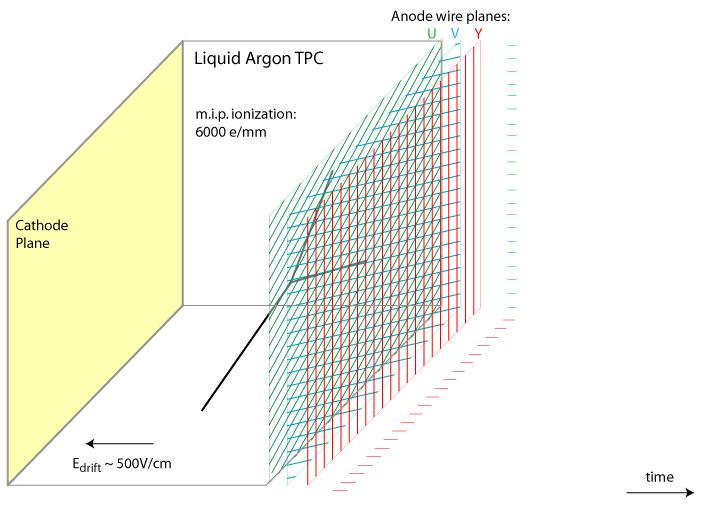
\includegraphics[width=0.9\textwidth]{signal-0.png}
	\caption{Liquid Argon TPC with wire readout: principle of operation}
	\label{fig:signal-0}
\end{figure}

The Liquid Argon Time Projection Chamber (LArTPC) is in essence a specially instrumented ionization chamber. Charges (electrons and positive ions)
created due to passage of ionizing particles through the sensitive medium (argon in this case) are subject to the effect of a uniform electrostatic
field which is created in Liquid Argon by a system of cathode and anode electrodes, which causes them to move (drift) along the field lines.
If there is an additional electrode within the Liquid Argon volume in the vicinity of the drifting charge, there will be a signal induced on it. Multiple such
electrodes (sensors) provide means for spatial characterization of the ionization charge distribution in the sensitive volume (which for example may
correspond to a particle track). Importantly, the shape of the signals on the electrode vs time is used to measure charge localization along the drift
direction (hence the term ``Time Projection Chamber''). For example, ionization electrons which are closer to the collection electrode will arrive to it sooner than
more distant ones, therefore time evolution of the signals on the affected wires will reflect distribution of the charge along the drift axis.

Current design of large scale LArTPC devices features planar arrays of wire electrodes supported by
rectangular frames. Such design contains an essential element called \textit{Anode Plane Assembly} (APA), which includes the ``collection plane'' (anode)
and two planes of sensor wires, called ``induction planes'', oriented at stereo angles with respect to each other and the collection plane.
Due to stereo angles, such arrangement allows for 2D measurement of the charge density distribution in the APA plane.
This is illustrated in Fig.~\ref{fig:signal-0}, which schematically shows the drift volume (to the left), the induction planes ``U'' and ``V'' and
the collection plane ``Y''. An important feature of such arrangement is that the \textit{same drifting charge} is measured three times as it
is detected by the three wire planes. This is further illustrated in Fig.~\ref{fig:3projections} as a schematic of drifting charge creating signals on wires,
represented conceptually as a view along the direction of the drift.

\begin{figure}[h!]
	\centering
	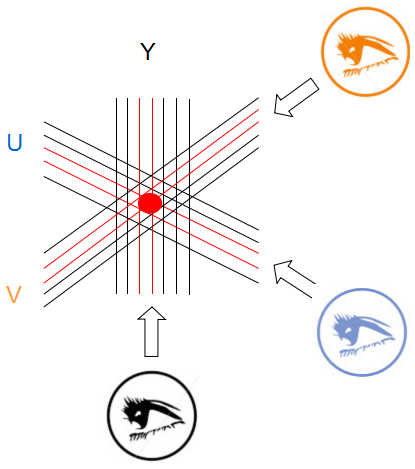
\includegraphics[width=0.65\textwidth]{uvy_2.png}
	\caption{Three projections of an object in a TPC with wire-based readout}
	\label{fig:3projections}
\end{figure}

Using just three projections to reconstruct an extended object (ionization charge density) presents challenges for event reconstruction.
Reliability and thorough characterization of the algorithms employed in this area will be critical for the systematics and other performance characteristics of DUNE.

There are a few approaches currenlty in development for event reconstruction. The ``Pandora'' toolkit (\ref{sec:pandora}), which
originated as R\&D for fine-grained calorimetry at ILC~\cite{pandora}, is being adopted to reconstruct LArTPC events.
In addition, there is a ``projection matching algorithm'' which will be used for test-beam studies with protoDUNE detector.

There is also a promising toolkit under development (called ``Wire Cell'') based on a different approach.
It performs three-dimensional imaging of events using the principles commonly applied in tomography.
As is frequently the case in tomographic reconstruction with sparse data, this may require the use memory- and CPU-intensive computing platforms.
It is likely that meeting the demands of such calculations will require adopting emerging technologies that are now becoming more common in
HEP, such as GPU or other co-processor acceleration and/or massively parallel systems such as HPC facilities.

\subsection{Pandora}
\label{sec:pandora}
 Pandora is a toolkit for implementing pattern recognition algorithms for fine-grain detectors, based on the so-called ``particle flow'' approach~\cite{pandora}.
It was conceived as a way to improve resolution of calorimetric measurements by taking advantage of the detector granularity. Pandora incorporates a
number of algorithms for different stages of event reconstruction, such as clustering algorithm, topological association algorithms, track-cluster association
algorithms and others, while providing a framework to utilize and manage these components. The framework also deals with memory management
and is designed to minimize external dependencies.

Pandora was adopted for event reconstruction in LBNE and now continues as a DUNE effort. It has been incorporated into the LArSoft sofware toolkit
as a package.



\subsection{Wire Cell}
\label{sec:wirecell}
\subsubsection{The Inverse Problem}

The LArTPC acts an imaging device, i.e. the physics information about the processes taking place in the detector volume is extracted by
analysing the 3D structures (images) of ionization patterns produced by particles participating in these processes. The only source of information
available for reconstruction of these images are amplitudes of signals coming from the wires in (U,V,Y) recorded as a function of time
as described above. It follows that the event reconstruction problem in DUNE TPC is a fairly typical case of the \textit{Inverse Problem},
where a 3D structure must be calculated based on a set of observables.

Because of time quantization inherent in operation of ADC, the 3D image effectively becomes an assembly of 2D slices.
In a given time slice, the 2D charge density distribution is observed via three different projections along the axes (U,V,Y) (see Fig.~\ref{fig:3projections}).
There is substantial similaritiy between this type of inverse problem and Computed Tomography (CT) with limited projection data. This similarity becomes even more prominent as we observe that in a
given slice the charge signals on wires are essentially linear integrals of the 2D charge density along each of the three observation axes. Common with many tomographic applications, the reconstruction strategy
then consists of calculating patterns in each 2D slice and then combining them into a full 3D structure. There are many event types and topologies
in DUNE, one example of a simulated neutral-current event in presented in Fig.~\ref{fig:ncc-example-1}.

\begin{figure}[h!]
	\centering
	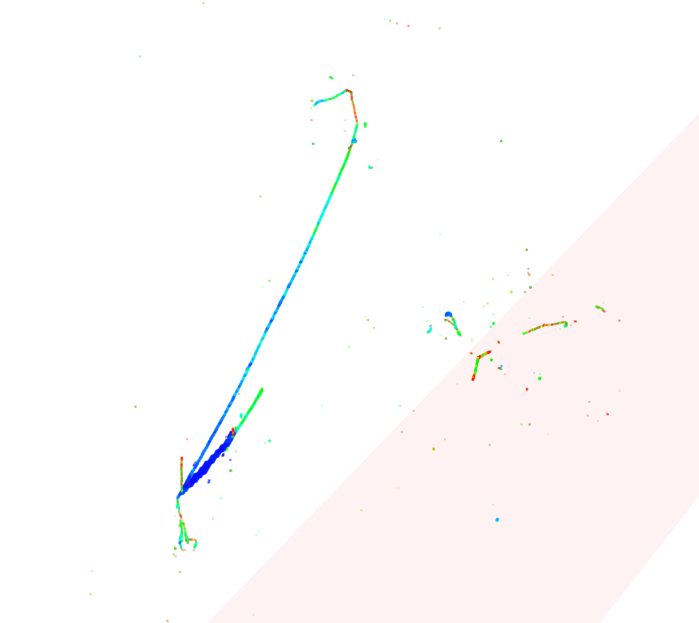
\includegraphics[width=0.7\textwidth]{ncc-example-1.png}
	\caption{An example of a neutrino-induced reaction in Liquid Argon ( simulation)}
	\label{fig:ncc-example-1}
\end{figure}

It's easy to see that (again, similar to majority of tomographic application) the reconstruction problem in DUNE is an ill-posed one,
due to the very limited set of just three observation angles. At the most basic level, this issue
manifests itself as ``ghost hits'' (well known in HEP), which is an ambiguity inherent in stereo
projection measurements.

The ``Wire Cell'' approach to this problem is based on the following:
\begin{itemize}
\item ``Voxelization'' of the TPC volume by treating each 2D slice as a tessellation (i.e. consisting of polygon-shaped tiles).

\item Solving an optimization problem which maximizes the likelihood of a given configuration of tiles (with charge associated with them) producing the observed signal distribution on the wires.

\item In reference to the optimization problem described above: regularization based on testing hypotheses about the object topology, e.g. that it's a track in a given portion of the volume. For example, cells in adjacent time slices can be tested for proximity in 2D.
\end{itemize}

To make this approach possible, there is one prerequisite that must be met, and that is a precise measurement of charge on each wire. This involves
proper calibration of the detector as well as solution of yet another inverse problem -- deconvolution of the detector and electronics reponse while
reconstructing the original shape of the charge signal. This is done in conditions of non-zero noise and involves applicaiton of digital filtering techniques.

\subsubsection{Wire Cell Components}
The flow of data in Wire Cell is presented in Fig.~\ref{fig:wirecell-diagram} in~\ref{sec:wc-diagram}.
Full description of Wire Cell is  beyond the scope and size limitations of this document,
so presented below is an annotated list of those elements of the data flow (see the diagram for specific
names) which are significant and/or present most computational challenges.
\begin{description}
\item[Slicer:] takes one "time frame" or a "readout" of raw data from DAQ (or simulated source)
and separates it in time bins.  Each bin contains ADC values for all the channels
(i.e. wires) with signal above a certain threshold that span the time bin.
	
\item[Cell Finder:] takes as a time bin and identifies ``cells'' (groups of adjacent tiles).
	
\item[Optimization Solver (``Matrix Solver''):] optimizes the likelihood of the charge contained in contiguous groups of cells
with respect to producing the observed signals on wires, utilizing a model where this relationship is expressed as a matrix.
	
\item[Clustering:] aggregates groups of cells over multiple time bins, thus creating 3D objects (``clusters'').
	
\item[Tracking:] connects clusters according to certain geometry rules, forming track candidates
	
\item[PID:] determines the type of particle based on ionization pattern, as defined by
charge depositions along the particle trajectory
\end{description}

\noindent
Elements listed above are computationally complex for a number of different reasons. For example,
the \textit{Cell Finder} performs a search on an array of tiles and given the large number
of those may face a combinatorial challenge. The \textit{Matrix Solver} has to solve an optimization
problem involving a sparse matrix. The \textit{Tracking} component has again to find relations
between multiple pieces of data based on applications of certain rules.
\newpage
\subsubsection{Wire Cell Diagram}
\label{sec:wc-diagram}
%\newpage
\begin{figure}[h!]
	\centering
	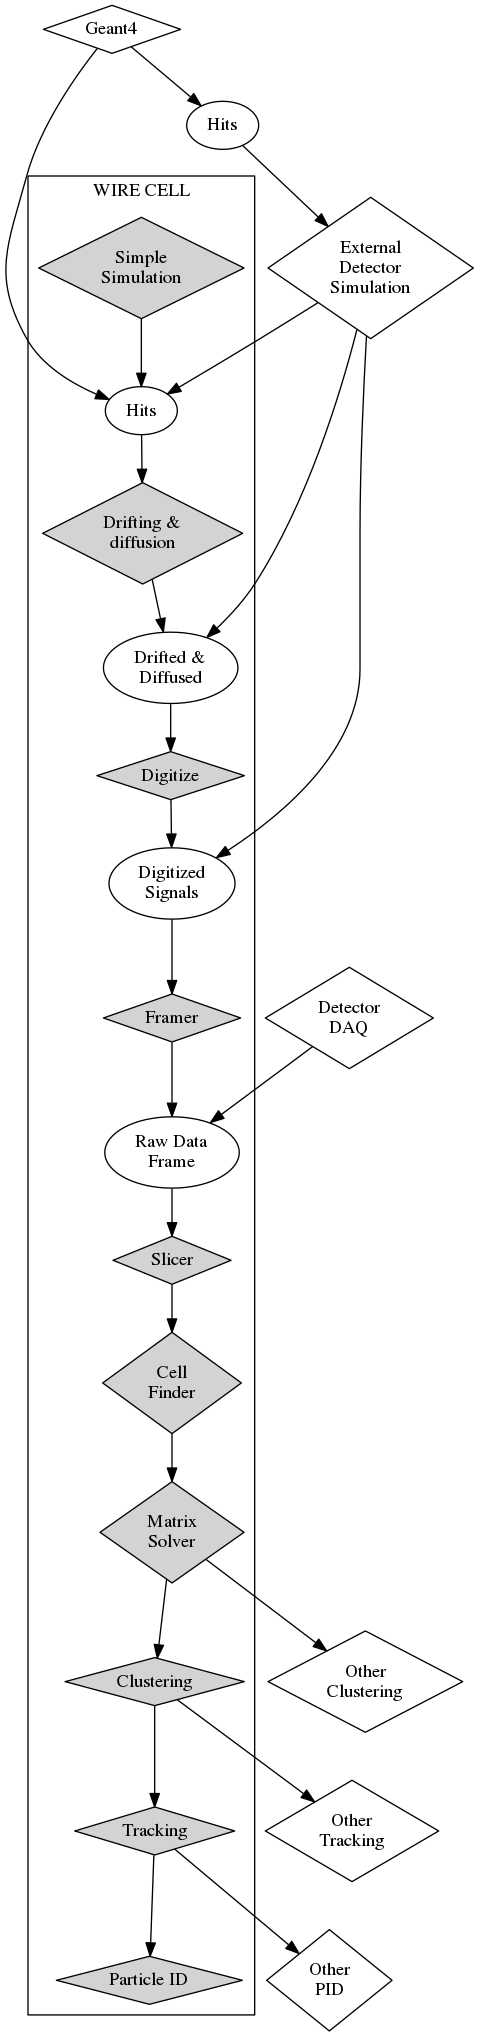
\includegraphics[height=0.8\textheight]{wirecell-dataflow-conceptual.png}
	\caption{Components of Wirecell Reconstruction Software}
	\label{fig:wirecell-diagram}
\end{figure}


\newpage


\newpage
% We can use verb tag to enter URL but it's better to use native url latex tag
\begin{thebibliography}{99}

\bibitem{sciopps} ``The Long-Baseline Neutrino Experiment: Exploring Fundamental Symmetries of the Universe'',  \url{http://arxiv.org/abs/1307.7335}

\bibitem{cdr_vol2} ``LBNF and DUNE Conceptual Design Report, Vol 2: The Physics Program for DUNE at LBNF'', \url{http://arxiv.org/abs/1512.06148}

\bibitem{cdr_vol4_docdb} LBNE\,DocDB\,10690  % \,\url{http://lbne2-docdb.fnal.gov/cgi-bin/DocumentDatabase/}

\bibitem{geant4} GEANT4: \url{https://geant4.web.cern.ch/geant4/}

\bibitem{mars} Official MARS site: \url{http://www-ap.fnal.gov/MARS/}

\bibitem{ar39endpoint} LBNE~DocDB~3018% \url{http://lbne2-docdb.fnal.gov:8080/cgi-bin/ShowDocument?docid=3018&version=3}

\bibitem{ar39bkg} ``Measurement of the specific activity of 39Ar in natural argon'', P. Benetti et al. Nucl.Instr. and Meth. A, vol. 574, p. 83, 2007.

\bibitem{atlas1collisions} ``Operating the ATLAS data-flow system with the first LHC collisions'', Journal of Physics: Conference Series 331 (2011) 022007

\bibitem{cms_daq} ``The New CMS DAQ System for Run-2 of the LHC'', IEEE TRANSACTIONS ON NUCLEAR SCIENCE, VOL. 62, NO. 3, JUNE 2015

\bibitem{bnl_protodune_data} \url{https://dune.bnl.gov/wiki/CERN_Prototype_Data_Handling}

\bibitem{slac_rce_1} \url{http://ldrd.slac.stanford.edu/accepted_proposals/2013/Convery.asp}

\bibitem{alice} \url{http://aliceinfo.cern.ch/Public/en/Chapter2/Chap2_TPC.html}

\bibitem{spade_icecube} IceCube\,Data\,Movement, \url{https://icecube.wisc.edu/science/data/datamovement}.

\bibitem{spade_dayabay}"Data processing and storage in the Daya Bay Reactor Antineutrino Experiment" M. He, Nucl. Phys. B Proceedings Supplement 00 (2015) 1–5 (\url{http://arxiv.org/abs/1501.06969}).

\bibitem{atlas_express} "Prompt reconstruction of LHC collision data with the ATLAS reconstruction software" N.Barlow et al, \textit{Journal of Physics: Conference Series 331 (2011) 032004}

\bibitem{pandora} ``The Pandora Software Development Kit for Particle Flow Calorimetry'', Journal of Physics: Conference Series 396 (2012) 022034

\bibitem{muon_bkgd_pdk} ``Muon-induced background to proton decay in the $p \rightarrow K^+\nu$ channel with large underground liquid argon TPC detectors'', \url{http://arxiv.org/abs/1504.06520}

\bibitem{kudr_bkgd_pdk} V.Kudryavtsev, private communication.

\bibitem{sam_chep12} ``Taking Global Scale Data Handling to the Fermilab Intensity Frontier'', Journal of Physics: Conference Series 396 (2012) 032069

\bibitem{monarc} \url{http://barone.web.cern.ch/barone/monarc/RCArchitecture.html}

\bibitem{lhc_model_update} \url{http://cds.cern.ch/record/1695401?ln=en}

\end{thebibliography}

\end{document}
